\documentclass{article}

% Language setting
% Replace `english' with e.g. `spanish' to change the document language
\usepackage[french,english]{babel}

% Set page size and margins
% Replace `letterpaper' with `a4paper' for UK/EU standard size
\usepackage[a4paper,top=2cm,bottom=2cm,left=3cm,right=3cm,marginparwidth=1.75cm]{geometry}


% Useful packages
\usepackage{amsmath}
\usepackage{graphicx}
\usepackage{svg}
\usepackage{hyperref}
\usepackage{xparse} % Required for handling optional/multiple macro arguments cleanly
\usepackage{float}
\usepackage{pdfpages}
\usepackage{caption}
\usepackage{listings}
\usepackage{minted}
\usepackage{booktabs}
\usepackage{longtable}
\usepackage{array}
\usepackage{multirow}
\usepackage[T1]{fontenc}
% \usepackage{showframe}
\usepackage[title]{appendix}
% \usepackage{todonotes} \setlength{\marginparwidth}{2cm}
% \usepackage{enumitem}
\usepackage{csquotes}
\usepackage[backend=biber, style=numeric, sorting=none]{biblatex}
\addbibresource{references.bib}


% Macros
% ESIR
\newif\ifdetails
\detailstrue
% \detailsfalse
% Research questions
\newcounter{rqcnt} % Counter
\renewcommand{\therqcnt}{RQ\arabic{rqcnt}} % Format the reference to 'RQn' instead of just 'n'
\newcommand{\formatRQ}[2]{
    \begin{quote}
        \textbf{#1:} \textit{#2}
    \end{quote}
}
\newcommand{\RQ}[2]{ % Register a new question
~\refstepcounter{rqcnt}\label{rq:#1} % Increment and set target for \label, then save ref label
    % Save the question text globally using a unique key name based on the ID
    \expandafter\gdef\csname stored@rq@#1\endcsname{#2} % chktex 41
    \formatRQ{\therqcnt}{#2}
}
\newcommand{\printRQ}[1]{ % Duplicate/reprint a stored question
    % Retrieve the number using standard~\ref, and text via our global storage macro
    \formatRQ{\ref{rq:#1}}{\csname stored@rq@#1\endcsname} % chktex 41
}
% Environments
\newenvironment{code}{\captionsetup{type=listing}}{}
\newenvironment{punctuationplit}{%
    \let\origunderscore\_
    \let\origdot\.
    \let\origcolon\:
    \let\origdash\-

    \newif\iffirstchar
    \firstchartrue

    \renewcommand{\_}{%
        \iffirstchar
            \origunderscore
            \firstcharfalse
        \else
            \discretionary{}{\origunderscore}{\origunderscore}%
        \fi
    }%

    \renewcommand{\.}{%
        \iffirstchar
            \origdot
            \firstcharfalse
        \else
            \discretionary{}{\origdot}{\origdot}%
        \fi
    }%

    \renewcommand{\:}{%
        \iffirstchar
            \origcolon
            \firstcharfalse
        \else
            \discretionary{}{\origcolon}{\origcolon}%
        \fi
    }%

    \renewcommand{\-}{%
        \iffirstchar
            \origdash
            \firstcharfalse
        \else
            \discretionary{}{\origdash}{\origdash}%
        \fi
    }%
}{}



% Settings
% \setlength{\parskip}{\baselineskip}
% \setlist[enumerate]{nosep}





\title{Studying LLM-assisted automated test generation for Machine Learning in Python}
\author{Théo \textsc{Ginguené}}

\begin{document}
\maketitle

\begin{abstract}
\dots

\end{abstract}

\ifdetails
\begin{otherlanguage}{french}
    \begin{abstract}
        \dots

    \end{abstract}
\end{otherlanguage}
\fi

\tableofcontents
\newpage

\section{Introduction}\label{sec:introduction}
Software testing is an essential part of software development, as it helps detect defects and provides evidence that software behaves as intended. Historically, this has been done manually, which can be tedious and time-consuming, particularly for large and complex software systems.
To address this issue, automated test generation tools have been created. Automated test generation aims to reduce this effort by automatically producing test cases that exercise the program under test. Among the different approaches to automated test generation, search-based software testing (SBST) formulates test generation as an optimization problem and uses search techniques, often evolutionary algorithms, to maximize a fitness criterion such as code coverage.
Many of them were first developed for Java, because of its widespread use in research and business, and its strong typing, simplifying the generation process.
One such example is Evosuite~\cite{ESECFSE11}, which uses an evolutionary approach based on genetic algorithms to automatically generate JUnit test suites.
However, some specific fields of computer science like machine learning often use Python, whose dynamic typing and highly flexible object model make the search space more difficult to explore. Using the same principles as Evosuite, Pynguin~\cite{Lukasczyk_Pynguin_Automated_Unit_2022} was then developed to cover this gap in test generation tools for Python.

The default algorithm these two tools use is called Dynamic Many-Objective Sorting Algorithm (DynaMOSA)~\cite{7840029}. DynaMOSA formulates branch coverage as a many-objective optimization problem and dynamically focuses the search on uncovered targets. While it has been shown to outperform its predecessors~\cite{7840029}, and although such approaches can generate effective test suites for many Python programs, they can struggle when reaching a coverage target requires constructing inputs satisfying complex constraints. This problem is particularly apparent in machine learning libraries, where functions often require structured inputs such as tensors, arrays, data frames, or objects satisfying implicit relationships between their values and attributes. Previous work on automated testing of machine learning libraries has shown that conventional test-generation techniques can achieve limited coverage and that providing structured input data can help reach code that is difficult to exercise through unconstrained search alone~\cite{Lucas_Berg_Improving_automated_unit_test_generation_for_machine_learning_libraries_using_structured_input_data_2024}. LLM-assisted approaches subsequently emerged as a complementary strategy to SBST.

Large Language Models (LLMs) offer a potential way of addressing this limitation. Unlike evolutionary search, an LLM can use source-code context, documentation, and learned programming knowledge to directly propose inputs and sequences of operations that satisfy non-trivial constraints. This makes LLMs particularly interesting as a complement to SBST: rather than replacing the search process, an LLM can provide promising test cases from which the evolutionary search can continue.

Combining LLMs and traditional approaches such as DynaMOSA has been shown to improve code coverage further than each method individually, in a new algorithm---CodaMOSA~\cite{10172800}. When the search reaches a coverage plateau, the algorithm asks an LLM to generate tests for under-covered parts of the program and uses these tests to redirect the search. A central challenge in this approach is the interface between the unrestricted code generated by the LLM and the restricted internal representation required by the search-based algorithm. The generated Python code therefore has to be parsed and transformed into test cases that can be manipulated by the SBST algorithm. This algorithm has been adapted in Pynguin, through the name of LLMOSA. The resulting approach is promising for machine learning libraries because it can combine the exploratory capabilities of evolutionary search with the ability of an LLM to construct complex inputs.


\ifdetails
\subsection{Context}
This paper is the result of a research internship at the SNAIL~\cite{snail_team} team of the University of Namur, in Belgium. The internship was supervised by Dr. Xavier Devroey.
The SNAIL~\cite{snail_team} team (Software Normalization Assessment and Improvement Lab) aims to help produce and identify quality software. The team is part of the Precise~\cite{precise_research_center} research center (Research Center in Information System Engineering), within the NADI institute~\cite{nadi} (Namur Digital Institute) of the University of Namur.

\fi

\subsection{Problem}
Because of the random nature of genetic algorithms, DynaMOSA has trouble trouble generating tests for machine learning (ML) libraries, for example scikit-learn or numpy~\cite{erni2024sbfttoolcompetition2024}. Some functions require complex data structures (\textit{e.g.} a pandas DataFrame with a column \texttt{col\_y} existing), which are hard to generate through evolution only, because that would require stumbling upon the required constraints randomly. LLMOSA seems like a promising alternative, because providing the code of the subject under test (SUT), an LLM can produce such data structures.
However, when trying to run LLMOSA on code oriented toward machine learning, a few problems occurred, making the LLM unable to generate tests.

As discussed in Section~\ref{sec:introduction}, to combine the LLM and DynaMOSA approaches, Pynguin deserializes the generated code from the LLM (a sequence of characters) into a list of test case chromosomes, a format used by the DynaMOSA algorithm to evolve the test cases. This conversion (as described in figure~\ref{fig:parser_diagram}) operates in two phases.
The rewriter first takes the LLM response, extracts code blocks and specifically Python functions named '\texttt{test\_\dots}', and transforms statements to make them easier to deserialize (\textit{e.g.} walrus expressions are transformed into regular assignments).
The deserializer then converts the simplified code into Pynguin's classes.

\begin{figure}[hbt!]
    \centering
    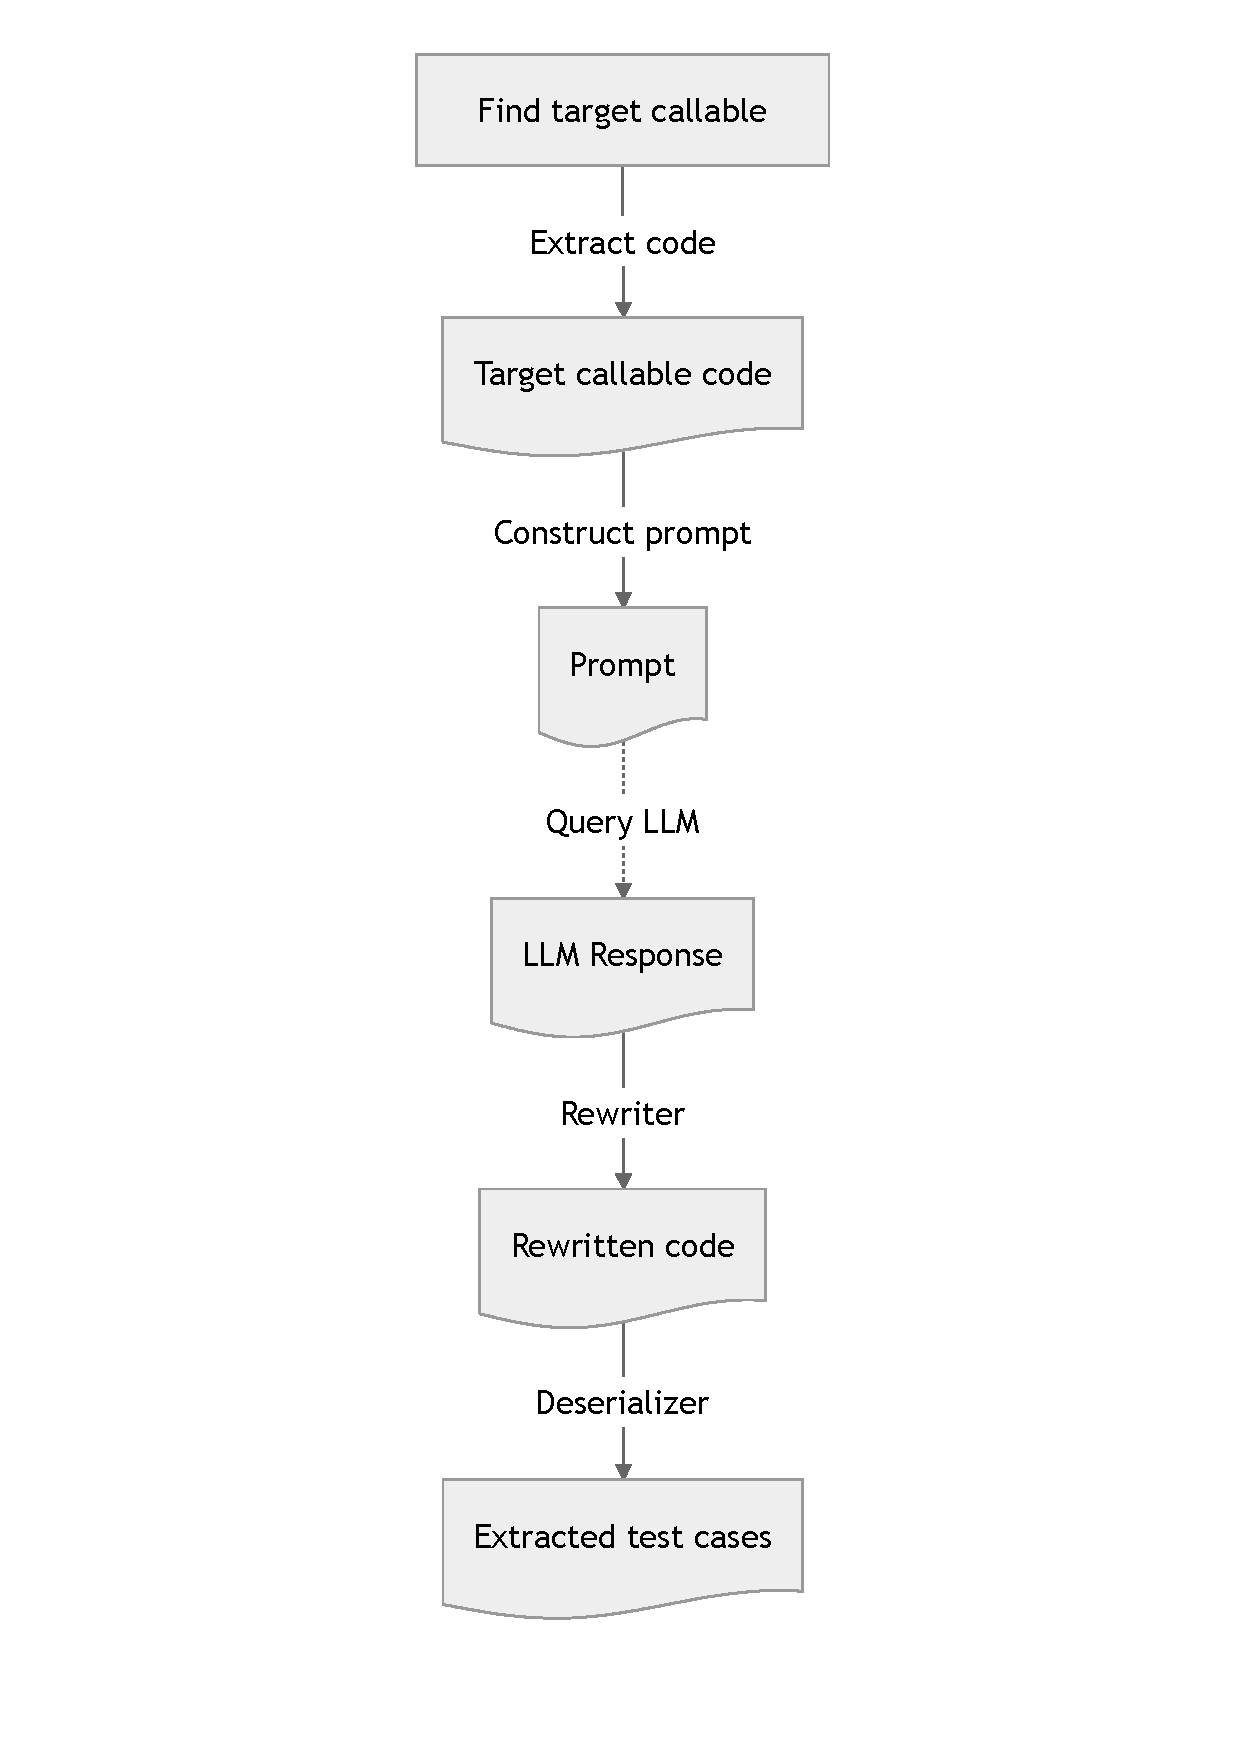
\includegraphics[width=0.5\linewidth]{assets/parser_diagram}
    \caption{LLM test generation sequence}\label{fig:parser_diagram}
\end{figure}

Each step adds uncertainty and potential errors.
This paper aims at solving these problems one by one, first explaining them, before solving them and evaluating the impact of these changes. Our goal is to investigate Pynguin's LLMOSA algorithm, in particular---though not only---for machine learning applications, and try to improve it. We will also try to evaluate the impact of different important parameters, such as the prompt used to generate the tests, and the model used to generate them.


\subsection{Contributions}
In this paper, we present the following contributions:

\begin{enumerate}
\item We introduce an extensible LLM-provider system and implement a local provider based on Ollama, enabling experiments with open-weight models without relying on an external API.
\item We propose an more detailed prompting and context-compression strategy designed to produce test cases that are both useful for SBST and compatible with Pynguin's test-case representation.
\item We improve the LLM-to-test-case pipeline by resolving imports from the module under test and by extending the rewriter and deserializer to support additional Python constructs and assertions.
\item We address several practical robustness issues encountered when applying LLMOSA to machine learning-oriented Python code, including interactions with native functions such as those exposed through pybind11.
\item We evaluate these changes experimentally on modules from several machine learning-related Python libraries, measuring their effects on code coverage and execution time and comparing different LLM models.
\end{enumerate}


\section{Background and related work}\label{sec:background}

\subsection{Search-based software testing}
Search-based software testing (SBST) formulates test generation as an optimization problem. The test generator searches for test cases that maximize a fitness function, usually code coverage. Evolutionary algorithms are particularly well suited for this type of tasks.

An example of this approach is EvoSuite, which automatically generates JUnit test suites for Java programs using evolutionary search~\cite{ESECFSE11}. EvoSuite demonstrated that search-based techniques can generate high-coverage test suites without requiring manually written tests. However, applying the same techniques to dynamically typed languages such as Python introduces additional challenges. In particular, the absence of static type information makes it more difficult to determine which objects can be used as arguments to a function and how those objects can be constructed.

Pynguin was introduced to address automated unit test generation for Python~\cite{Lukasczyk_Pynguin_Automated_Unit_2022}. It supports several search-based test-generation algorithms, including MIO, MOSA, and DynaMOSA. An empirical study found that evolutionary approaches outperform random test generation for Python programs, with DynaMOSA achieving the highest coverage among the evaluated approaches~\cite{Lukasczyk_Pynguin_Automated_Unit_2022}. Nevertheless, the study also identified type inference and the construction of appropriate objects as fundamental limitations for automated test generation in Python.

DynaMOSA extends the many-objective optimization approach by dynamically selecting the coverage targets that should guide the search~\cite{7840029}. Rather than optimizing all coverage targets equally throughout the entire search, DynaMOSA focuses computational effort on targets that are currently relevant. This makes the search more efficient, but it does not fundamentally solve the problem of constructing inputs that satisfy complex constraints. If reaching a branch requires a particular combination of values, object attributes, or method calls, evolutionary mutation may have a very low probability of discovering the required sequence.

This limitation is particularly relevant to the machine-learning ecosystem. A function may require not only an object of a particular type, but also an object satisfying constraints on its structure and contents. For example, a function may require a pandas DataFrame containing a particular column, a tensor with a specific shape and dtype, or an estimator that has previously been fitted. Such constraints make the search space much harder to explore.

For a more in-depth understanding of search-based software testing (SBST), specificially for machine learning applications, we refer the reader to Chapter 2 of Lucas Berg's thesis~\cite{Lucas_Berg_Improving_automated_unit_test_generation_for_machine_learning_libraries_using_structured_input_data_2024}, explaining in detail the different SBST approaches, test-case generation, fuzzing, and ML-specific testing.

\subsection{Automated testing of machine-learning software}
Machine-learning software introduces specific testing challenges. ML libraries manipulate structured numerical data and expose APIs with constraints involving tensor shapes, data types, dimensions, model states, and relationships between multiple inputs.

Previous work has therefore investigated specialized approaches for testing machine-learning libraries. In particular, structured input generation has been proposed as a way to improve automated unit-test generation for ML-oriented Python software~\cite{Lucas_Berg_Improving_automated_unit_test_generation_for_machine_learning_libraries_using_structured_input_data_2024}. Instead of relying exclusively on unconstrained search to construct complex objects, structured generators can provide inputs that already satisfy part of the constraints required by the API. This allows the search algorithm to spend more of its budget exploring program behaviour rather than discovering the representation of valid inputs.

Other approaches to ML testing have focused on fuzzing and domain-specific properties. These techniques can be effective when suitable transformations or invariants can be defined, but they generally require domain-specific knowledge about the software under test. This creates a complementary problem to SBST: while search-based techniques can automatically optimize coverage, they may lack the semantic knowledge required to construct meaningful inputs.

The problem can therefore be viewed as a mismatch between two capabilities. SBST provides an effective mechanism for exploring a program once suitable test cases exist, whereas generating the suitable test cases may require knowledge of API and implicit input constraints. This observation motivates the use of techniques capable of extracting such information from source code and documentation.

\subsection{Large language models for test generation}
Large Language Models (LLMs) provide an alternative way of generating test cases by exploiting their ability to process source code and produce executable programs. Unlike traditional search-based techniques, an LLM can directly infer relationships between function parameters, API calls, object construction, and expected behaviour from the textual representation of a program.

Recent research has consequently investigated the use of LLMs for automated test generation. These approaches differ in how much program information is provided to the model and how generated tests are validated or repaired. A central challenge is that LLM generated tests are not necessarily executable or useful for increasing coverage. Generated tests may contain incorrect imports, invalid API calls, missing dependencies, or assertions that do not correspond to the actual behaviour of the program.

Prompt design and program context are therefore important components of LLM-based test generation. Providing more source code can give the model additional information, but also increases the context size and generation cost. Conversely, aggressively reducing the context may remove information required to construct valid inputs. Recent work on code-aware prompting has investigated how program analysis and coverage information can be incorporated into LLM prompts to guide test generation more effectively~\cite{ryan2024codeawarepromptingstudycoverage}.

\subsection{Combining LLMs and search-based test generation}
Rather than replacing SBST, LLMs can be used to provide promising seeds for an existing search process. This approach combines the semantic knowledge of an LLM with the systematic exploration capabilities of evolutionary algorithms.

CodaMOSA is a representative example of this approach~\cite{10172800}. It integrates an LLM into a search-based test-generation process and invokes the model when the search reaches a coverage plateau. The LLM is asked to generate tests targeting under-covered parts of the program, and the resulting tests are then used to redirect the evolutionary search. In an evaluation over 486 benchmarks, CodaMOSA achieved statistically significant coverage improvements over both SBST and LLM-only baselines on substantially more benchmarks than those on which it reduced coverage~\cite{10172800}.

The CodaMOSA results suggest that the two approaches are complementary. SBST is effective at exploiting promising regions of the search space, but can become trapped when its mutations are unlikely to discover qualitatively different inputs. LLMs can instead make larger semantic jumps by proposing new sequences of operations or structured inputs. However, this advantage comes at the cost of relying on generated source code that must be correctly interpreted by the underlying test-generation framework.

This interface is particularly important for Python because of its dynamic nature and the large number of possible runtime objects. In Pynguin's implementation, LLM-generated tests are first rewritten and then deserialized into Pynguin's internal test-case representation.

\subsection{Positioning of this work}
The existing literature establishes three relevant observations. First, SBST can generate high-coverage tests for Python, but dynamically typed code makes type inference and test-input construction difficult~\cite{Lukasczyk_Pynguin_Automated_Unit_2022}. Second, machine-learning libraries amplify this difficulty because useful inputs frequently have structural and semantic constraints that are difficult to discover through unconstrained mutation~\cite{Lucas_Berg_Improving_automated_unit_test_generation_for_machine_learning_libraries_using_structured_input_data_2024}. Third, LLMs can provide useful test cases based on the code semantics, and approaches such as CodaMOSA demonstrate that combining LLM generation with SBST can improve coverage~\cite{10172800}.

Our work focuses on the practical interface between an LLM and Pynguin's search-based test generation. In particular, we investigate the effect of prompt design, context compression, LLM model selection, and improvements to the rewriting and deserialization pipeline. We additionally study these techniques on modules from machine-learning-related Python libraries, where structured inputs and native extensions introduce challenges that are less prominent in conventional Python benchmarks.

The objective is therefore not simply to determine whether LLMs can generate valid unit tests. Instead, we investigate which components of an LLM-assisted SBST pipeline contribute to effective coverage-oriented test generation, and under which conditions these components provide measurable benefits.


\section{Approach}\label{sec:approach}
Before trying to improve LLMOSA, the first step was trying to run it on a code sample.
We wrote an example of a code sample requiring specific input data structure (listing~\ref{lst:tab}) using pandas~\cite{The_pandas_development_team_pandas-dev_pandas_Pandas}, a popular library for data analysis.

\begin{code}
\caption{Module under test (MUT)}\label{lst:tab}
\begin{minted}[linenos, breaklines, frame=single]{python}
import pandas as pd

def process_df(df: pd.DataFrame) -> bool:
    '''Applies different operations to a DataFrame, in place.'''
    df.drop(columns=['col1'], inplace=True) # Requires col1 to exist
    return df.empty
\end{minted}
\end{code}

This sample has two different output to be tested, \texttt{True} and \texttt{False}.
The objective is to produce both compliant and non-compliant inputs to test this module. Non compliant outputs are relatively easy to generate, as any non DataFrame input will do. However, generating a compliant input is more difficult, as it requires a DataFrame with a column named \texttt{col1}, and another column, empty or not. This is an example of a function that is hard to test with DynaMOSA, but \emph{should} be easy to test with LLMOSA.

To test this, we tried running both DynaMOSA and LLMOSA on this module, with the default configuration.
However, running pynguin with LLMOSA required an OpenAI API key, which has the following drawbacks:

\begin{enumerate}
    \item Consistency: OpenAI can discontinue access to a specific model at any time, making it difficult to reproduce experiments. Open weights models can be downloaded, stored and used at any time for a better comparison and reproducibility, providing more stable results and full control over the model.
    \item Price: When benchmarking or through intensive use, cloud models token use can quickly add up to substantial expenses. Their prices are also subject to change, which may make it difficult to reproduce experiments later.
\end{enumerate}

For industrial purposes, it is also important to be able to run the tests locally, without relying on an external provider. This is particularly relevant for sensitive code, where sending it to a third-party provider may not be acceptable.

\subsection{New providers}
To reduce this dependency to an external provider, we decided to refactor the LLM logic and add support for a new provider, Ollama. This provider can be used to run open models~\cite{Ollama} locally, solving the issues raised above.
A configuration entry was added; \texttt{--provider}, taking as possible values the enum \texttt{LLMProvider}---currently \texttt{OPENAI} or \texttt{OLLAMA}.


\subsection{Prompt engineering}
Due to the constraints of the rewriter, we noticed that the LLM often failed to provide an appropriate structure. The prompt was minimalist and did not provide strong guidance to the LLM (listing~\ref{lst:original_prompt}).

\begin{code}
\caption{Original prompt}\label{lst:original_prompt}
\begin{minted}[breaklines, frame=single]{text}
Write unit tests for the following callables that Pynguin failed to cover:
{callables_section}
Module path: `{self.module_path}`
Module source code: `{self.module_code}`
\end{minted}
\end{code}

To try and guide the LLM towards providing a correctly structured response, we listed the requirements to satisfy for the rewriter to work:

\begin{enumerate}
    \item The answer should be inside a code block:\\
        Pynguin uses the regex \verb!r"```python([\s\S]+?)(?:```|$)"! to extract the code block from the LLM response. If the answer is not inside a code block annotated with triple backticks and ``python'', it will not be parsed.
        If no code block is found, the rewriter will return an empty list of test cases, which will make the algorithm fail to generate any test case.
    \item Each function must be named '\texttt{test\_\dots}':\\
        The rewriter specifically checks if the function name starts with '\texttt{test\_}'. If it does not, the function will be ignored and not parsed. It also has to either be top-level or inside a top-level class, but not inside another function or nested class.
    \item Each function must have no arguments:\\
        While the rewriter can handle functions with arguments, the deserializer cannot, due to the fact that Pynguin's test case representation does not support arguments. If a function has arguments, it will be ignored and not parsed. Without changing the whole test case representation, this requirement cannot be lifted.
    \item Pytest features (\textit{e.g.} fixtures) are not supported:\\
        Again, due to the limitations of Pynguin's test case representation, the deserializer cannot handle pytest features. Decorators in general are not rewritten, and will be ignored (except for \texttt{@pytest.mark.parametrize}, as explained below).
\end{enumerate}

We added a bit of context, and complementary instructions such as:
\begin{enumerate}
    \item Not rewriting the SUT's code, for three main reasons:
        first, it would skew pynguin's code coverage results, as the tests would not run on the SUT's actual code but on the rewritten version;
        second, it would make the tests less maintainable, as they would have to be updated if the SUT changes;
        third, it saves tokens and run time, which is beneficial for the overall efficiency of the testing process.
    \item Following the Arrange, Act, Assert pattern, which is a common pattern in unit testing. It helps to structure the tests and makes them easier to read and understand, which is useful for debugging and guides the LLM toward generating higher quality tests.
\end{enumerate}

All these instructions were compiled into a new prompt (listing~\ref{lst:our_prompt}), with an emphasis on the fact that the functions should have no arguments, because this was the main cause of parsing failures, and an example of a valid test function.
To help with running the same test with different values, we also added support for \texttt{pytest.\allowbreak{}parametrize}. We rewrite the decorated function as one function per parameter, with the parameter initialized at the start of the function body. This allows the LLM to use \texttt{pytest.\allowbreak{}parametrize} to generate multiple tests with different values, while still satisfying the requirement of having no arguments.

\begin{code}
\caption{Our prompt proposition}\label{lst:our_prompt}
\begin{minted}[breaklines, frame=single]{text}
You are writing tests to be used as seed for a SBST algorithm. Your goal is to improve as much as possible the coverage of the tests.
Write unit tests for the following callables that Pynguin failed to cover:
{callables_section}
Module path: `{self.module_path}`
Module source code:
```python
{compressed_module_code}
```
You answer will be parsed for mutations, so here are the guidelines you need to follow:
- Answer in a code block only using; one function for each test case, with NO ARGUMENTS, NO HELPER FUNCTIONS AND NO CLASSES.
- If needed, instantiate vars in the body of the test func or use pytest.parametrize, but DO NOT USE ANY OTHER PYTEST FEATURE (e.g. DO NOT USE FIXTURES), as that will make the parsing fail.
- Do not rewrite the SUT's code in the tests. If you want for example to call a function or instanciante a class, import it.
- Think first then answer in simple, concise assertion tests, split in small functions. Follow the Arrange, Act, Assert pattern.

Here are some examples; *NEVER DO*:
def func_all_tests(param):
    var0 = param
    ...

*INSTEAD DO*:
I need to test the function `func` that takes a parameter and returns a value. I will test the following scenarios: ...
```python
from module_to_test import func
def test_feat1():
    var0 = ...
    var1 = func(var0)
    assert ...
```

REMEMBER: NO ARGUMENTS IN YOUR TEST FUNCTIONS (if you don't use pytest.parametrize)"
\end{minted}
\end{code}

Naturally, the question that arises is the following:
\RQ{prompt}{Can our prompt improve the algorithm performance?}

Our prompt uses more tokens than the original one, however it is more specific and provides more guidance to the LLM. It is therefore expected to improve the algorithm performance, but it is not guaranteed.
We will try to find out and answer this question in section~\ref{sec:eval}.


\subsection{Regex}
As mentionned above, the rewriter uses a regex (\verb!r"```python([\s\S]+?)(?:```|$)"!) to extract the code block from the LLM response. We modified this regex to make it more robust, and to allow for more variations of the code block. The new regex is \verb!r"```py(?:thon)?([\s\S]+?)(?:```|$)"!, which allows for the code block to be annotated with both ``python'' and ``py'', as both are considered correct, and the LLM often uses the latter.

\subsection{Adding imports}
After adding the new prompt, we were able to consistently generate correct rewritten tests. When deserializing though, lots of statements got lost in the process: function calls, some asserts, attributes, some comparisons, \textit{etc}.
To illustrate this, we show a sample of the rewritten output (listing~\ref{lst:rewritten_output}) and the deserializer result (listing~\ref{lst:deserializer_result}).

\begin{code}
\caption{Rewritten output (sample)}\label{lst:rewritten_output}
\begin{minted}[breaklines, linenos, frame=single]{python}
def test_process_df_with_missing_values():
    var_0 = 'Test for a DataFrame with missing values.'
    var_1 = 'col1'
    var_2 = 'col2'
    var_3 = 1
    var_4 = 2
    var_5 = None
    var_6 = [var_3, var_4, var_5]
    var_7 = 3
    var_8 = [var_3, var_4, var_7]
    var_9 = {var_1: var_6, var_2: var_8}
    df = pd.DataFrame(var_9)
    var_10 = process_df(df)
    var_11 = True
    var_12 = var_10 is var_11
    assert var_12
\end{minted}
\end{code}

The deserializer result is missing many statements from the rewritten output, which is a problem for the algorithm's performance. The most important missing statements are the function calls, which are the main part of the test case. Without them, the test case is useless as it does not execute a single line of code from the SUT.

\begin{code}
\caption{Deserializer result}\label{lst:deserializer_result}
\begin{minted}[breaklines, linenos, frame=single]{py}
def test_generated_function():
    str_0 = 'Test for a DataFrame with missing values.'
    str_1 = 'col1'
    str_2 = 'col2'
    int_0 = 1
    int_1 = 2
    none_type_0 = None
    list_0 = [int_0, int_1, none_type_0]
    int_2 = 3
    list_1 = [int_0, int_1, int_2]
    dict_0 = {str_1: list_0, str_2: list_1}
    bool_0 = True
\end{minted}
\end{code}

After further investigation, we figured that the main cause of parsing failures was the impossibility to resolve objects from the libraries used by the test suite, including from the MUT (\textit{e.g.} \texttt{pd.DataFrame}, \texttt{process\_df}). Each unparsed statement then in turn caused the parsing of the subsequent statements to fail.
Two options were considered:
\begin{enumerate}
    \item\label{item:llm_imports} Gather the imports written by the LLM, import the corresponding libraries and search for matches in the imported objects.
    \item\label{item:mut_imports} Search in the libraries imported from the module under test (MUT).
\end{enumerate}

Option~\ref{item:llm_imports} makes sure that libraries explicitely cited by the LLM are imported, but has other implications, such as making sure that the package is installed, performance issues, and more unpredictable behavior.
That is why we opted for option~\ref{item:mut_imports}. This choice is further justified by the fact that most of the time, it is not required to import libraries other than those used by the MUT. We still added the imports hinted by the LLM in the rewriter, both for debugging purposes and easing the implementation of option~\ref{item:llm_imports} if necessary.

\subsection{pybind11 functions}
pybind11~\cite{pybind11} is a library that allows to create Python bindings for C++ code. It is used in many machine learning libraries, such as PyTorch, to expose C++ functions to Python.
However, pybind11 functions are not regular Python functions, and would make pynguin crash when trying to retreive their AST, because they reference an unreachable module.
This was fixed by setting the module tree to \texttt{None} when the module is not found.

\subsection{Statement fixes}
Even after adding the imports, even though the majority of statements were deserialized correctly, some still failed to be deserialized. We identified a few causes:

\subsubsection{Asserts}
Asserts were not added to the test case due to an incorrect configuration. If the assertion generator was not set to \texttt{AssertionGenerator.LLM}, the deserializer would not add asserts to the test case. However, the LLM was still generating asserts, which were then ignored by the deserializer. This was fixed by simply always adding asserts to the test case.

\subsubsection{Unary not}
Unary not statements (\textit{i.e.} \texttt{a = not b}) were not deserialized because the deserializer was not handling them. We added a special case checking for the not operator and creating the appropriate \texttt{ASTAssignStatement}.
This single change improves the deserializer success rate significantly because the LLM often uses the not operator in its generated code, especially when asserting that a boolean value is False (\textit{e.g.} \texttt{assert not df.empty}).

\subsubsection{Equality between variable references}
A problem in the implementation of the deserializer (when testing equality between variable references, \textit{e.g.} \texttt{z = x == y}) was causing it to crash on some occurences, stopping completely the test generation. The problem was later found and a patch was added in the main branch of Pynguin by the maintainer~\cite{VariableRefAST.structural_eq_fix}. Therefore, we did not include this problem fix in our comparison, as it is already available in the main branch of Pynguin.

\subsection{Evaluation}
After implementing all the changes above, we ask ourselves to which extent the changes impact the algorithm performance. We will try to answer the following research question:

\RQ{approach}{Is our new generation approach more effective?}
The evaluation will be done in section~\ref{sec:eval}.

\subsection{Compressing context}
The fixed deserializer was able to parse the rewritten output correctly, but when testing LLMOSA on a large module, we ran into issues. The LLM was often unable to generate a proper response. Sometimes it would time out, while other times it would a response that was not parsable by the rewriter or deserializer or simply unusable.
The run time also increased significantly, as the LLM had to process a lot of information.
We identified that the main cause of this problem was the context size. The LLM was given too much information---the entire module code, which could be very large, and the list of callables to cover, which could also be large (often the entire module).
To solve this problem, we implemented a context compression algorithm.

Using the module's AST, we can identify the callables we want to cover, and extract only the relevant code for each callable (\textit{e.g.} the class the callable belongs to). The other callables are then removed from the prompt (and replaced with a ``\mintinline{python}|# [...]|'' comment to hint that they were removed). This way, the LLM is given only the relevant information for each callable. We also limited the number of callables to cover in each prompt, to avoid giving too much information to the LLM.

We consider this compression algorithm as part of the prompt engineering, as it is a way to improve the prompt by reducing the context size.
As such, we will evaluate its impact on the algorithm performance in section~\ref{sec:eval} to try and answer \ref{rq:prompt}.

\subsection{Generating function parameters}
One of the main issues with SBST is the difficulty of randomly stumbling across valid function parameters. To adress this issue, we implemented a system to generate function parameters using an LLM. The LLM is given the function signature and docstring, and is asked to generate valid parameters for the function. The generated parameters are then used to call the function in the test case.

\begin{figure}[H]
    \centering
    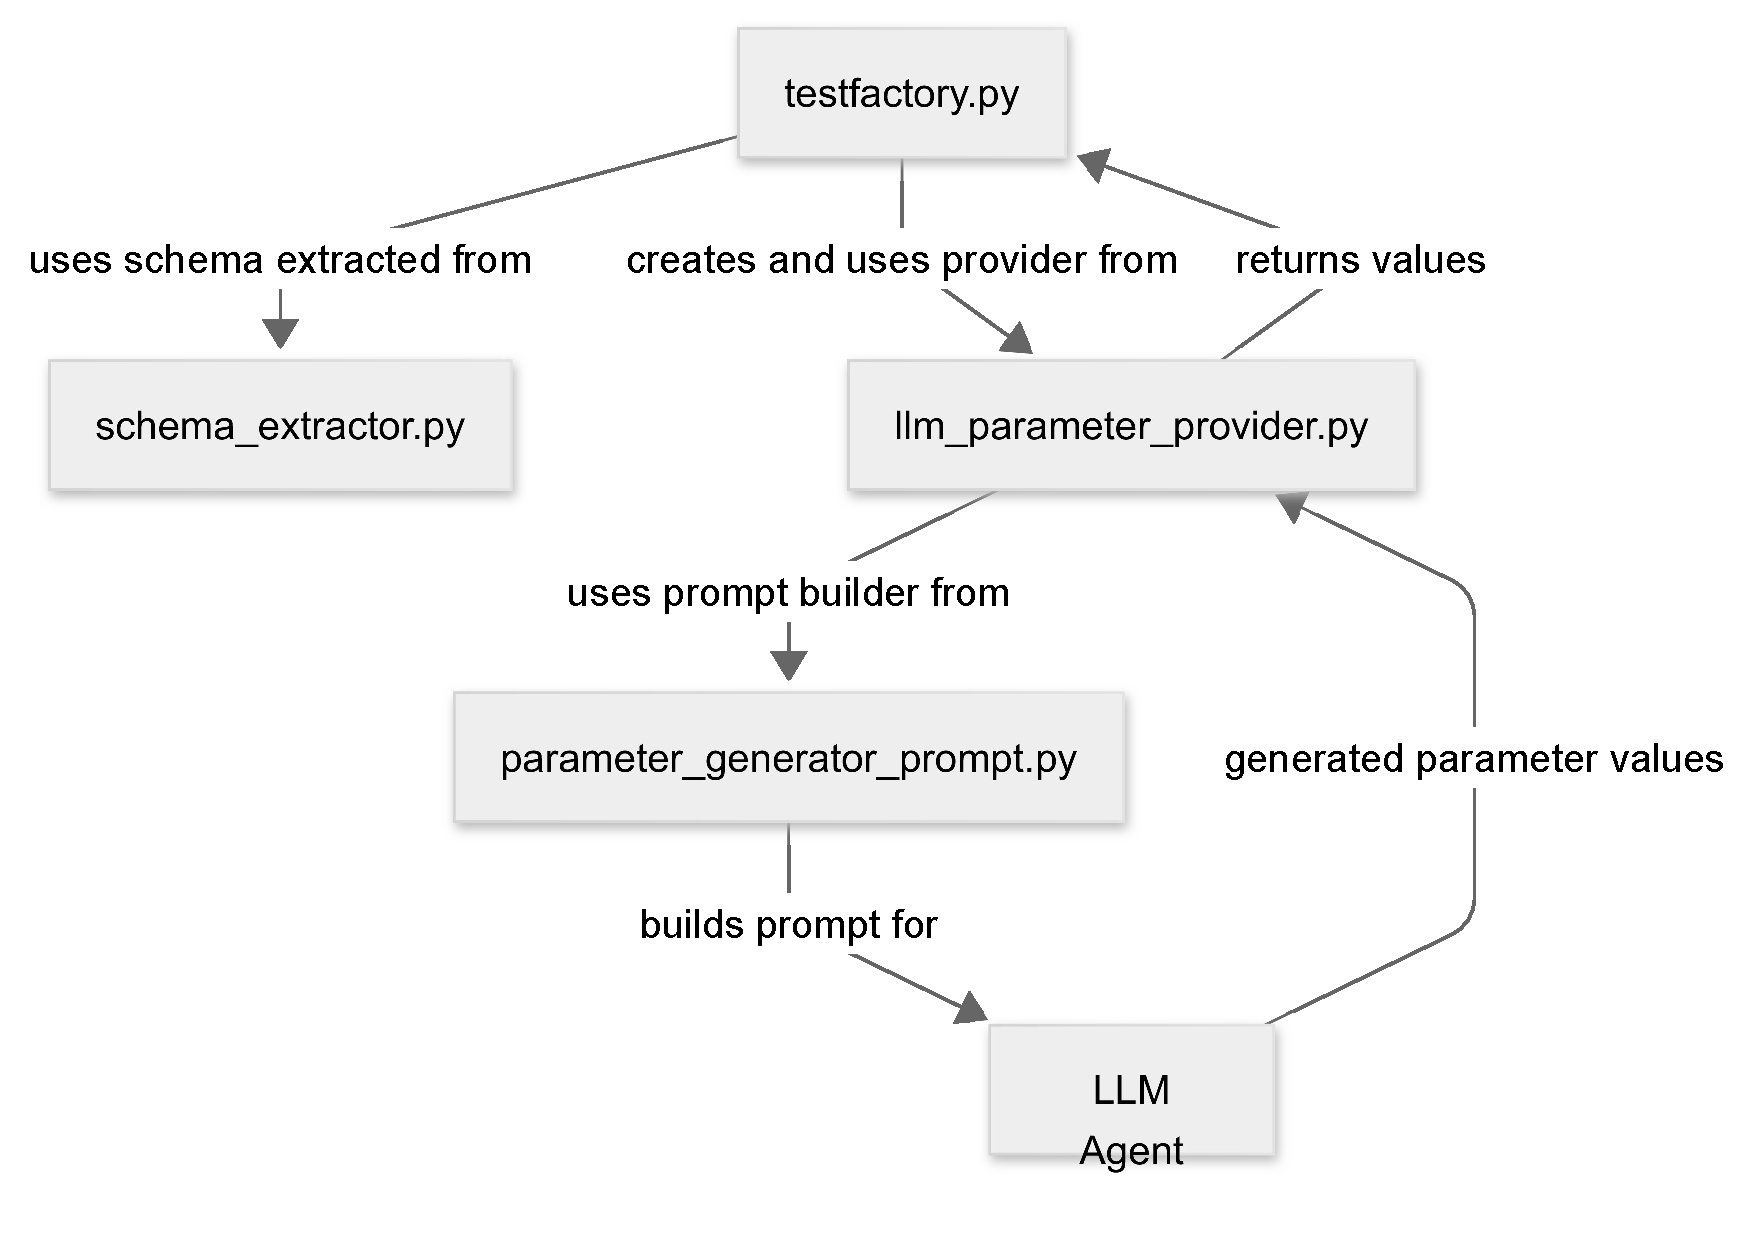
\includegraphics[width=0.5\linewidth]{assets/parameter_generator.pdf}
    \caption{Parameter generation flow}\label{fig:parameter_generator}
\end{figure}

Due to the fact that this system is still in development and the time constraints, this feature was not evaluated.

\section{Evaluation}\label{sec:eval}
To evaluate the impact of our changes on the algorithm performance, we ran a series of experiments on a set of modules from popular machine learning libraries. We compared the original approach with our new approach, and the original prompt with our new prompt, as well as comparing different models. The experiments were run on a compute cluster using Kubernetes, with each experiment running in a separate pod. Each experiment was run 30 times to account for the randomness of the algorithm, and the results were collected and analyzed.

We used the Mann--Whitney U test because each experiment contains independent runs of a randomized algorithm, and we report the Vargha--Delaney effect size $\hat A_{12}$ in addition to the $p$-value, according to the recommendations of Arcuri and Briand~\cite{10.1145/1985793.1985795}. An effect size close to $0.5$ indicates that the two configurations perform similarly. In all comparisons, $\hat A_{12}$ is oriented so that values above $0.5$ favor the left-hand configuration: for coverage score this means a larger score, while for duration the values are reversed, so it means a shorter execution time. Values below $0.5$ therefore favor the right-hand configuration.

When we later refer to the ``score'', we mean the coverage score, which is the main metric used to evaluate the performance of the algorithm. The coverage score is a value between 0 and 1, representing the percentage of code covered by the generated tests. A higher score indicates better performance.
While it is not a perfect representation of a test suite's quality, it is a good indicator of the algorithm's performance and one of the easiest metrics to measure. It is also the main metric used in most papers about automated test generation.

\subsection{Dataset}
Considering the goal of this paper is to improve LLMOSA for machine learning applications, we selected a few modules from popular machine learning libraries.
We selected modules from pytorch, TabGAN, and transformers, which are popular libraries for deep learning and natural language processing.
They were selected randomly between libraries that had a wide range of complexity and popularity, and that covered different aspects of machine learning, such as neural networks, tabular data generation, and natural language processing.
All these libraries are part of the Awesome Python list~\cite{Awesome_Python}, which is a curated list of Python frameworks, libraries, tools, and resources.
The modules were selected randomly from the libraries, to avoid any bias in the selection process.
Here are the exact modules we used in our benchmark, with their path in the library:
\begin{itemize}
    \item \texttt{pytorch/torch/\_numpy/\_ndarray.py}
    \item \texttt{pytorch/torch/\_numpy/\_getlimits.py}
    \item \texttt{pytorch/torch/nn/attention/bias.py}
    \item \texttt{pytorch/torch/nn/attention/flex\_attention.py}
    \item \texttt{Tabular-data-generation/src/\_ForestDiffusion/diffusion\_with\_trees\_class.py}
    \item \texttt{Tabular-data-generation/src/tabgan/adversarial\_model.py}
    \item \texttt{Tabular-data-generation/src/\_ctgan/transformer.py}
    \item \texttt{transformers/src/transformers/tokenization\_utils\_base.py}
    \item \texttt{transformers/src/transformers/pipelines/text\_generation.py}
    \item \texttt{transformers/src/transformers/data/metrics/squad\_metrics.py}
    \item \texttt{pytorch/torch/nn/modules/rnn.py}
    \item \texttt{pytorch/torch/\_numpy/\_util.py}
    \item \texttt{pytorch/torch/\_numpy/\_funcs.py}
    \item \texttt{pytorch/torch/\_numpy/\_ufuncs.py}
    \item \texttt{pytorch/torch/\_numpy/\_normalizations.py}
\end{itemize}

\subsection{Experiment setup}
We want to answer the following research questions:
\printRQ{prompt}
\printRQ{approach}

To answer~\ref{rq:approach}, we ran the experiments with the original approach and our new approach, both with the same configuration and using LLMOSA. We called this experiment ``classic''.

To answer~\ref{rq:prompt}, we ran the experiments with the default prompt, our new prompt with context compression (``UncoveredTargetsPrompt''), and the same new prompt without context compression (``NoCompressionPrompt''), again keeping the remaining configuration unchanged. We called this experiment ``prompt''.

We also introduce a new question, which is not directly related to our changes, but is interesting to investigate: \RQ{model}{Which model(s) performs best?}
To answer~\ref{rq:model}, we ran the experiments with the same configuration and using LLMOSA, but with different models. We compared the performance of the following models, chosen to vary in size, specific capabilities, and model family:
\begin{itemize}
    \item \texttt{qwen2.5:1.5b}
    \item \texttt{qwen2.5:3b}
    \item \texttt{qwen2.5-coder:0.5b}
    \item \texttt{qwen2.5-coder:1.5b}
    \item \texttt{qwen2.5-coder:3b}
    \item \texttt{qwen2.5-coder:7b}
    \item \texttt{qwen3:4b}
    \item \texttt{qwen3.5:4b}
    \item \texttt{gemma4:e2b}
    \item \texttt{gemma4:12b}
    \item \texttt{gemma4:26b}
    \item \texttt{gemma4:31b}
\end{itemize}

\subsubsection{Containerization}
We deployed our experiments in a compute cluster using Kubernetes. A job was created for all experiments, which created a pod for each experiment. Each pod was running a container, which contained all the dependencies required to run the experiments. The container was built using a Dockerfile, which installed all the dependencies and copied the source code of our project into the container. The Dockerfile was optimized to improve the build time, as the installation of the dependencies was the most time consuming part of the build process.


\subsubsection{Configuration}
As per the recommendations of Arcuri and Briand~\cite{10.1145/1985793.1985795} on statistical tests for assessing randomized algorithms, and because of the time needed to run the benchmark (up to a few hours per experiment), we ran each experiment 30 times on each one of the 15 modules to account for the randomness of the algorithm. The configuration of the experiments was the default configuration of Pynguin, with the following changes:
\begin{itemize}
    \item provider: Ollama
    \item algorithm: LLMOSA
    \item model-name: See for each experiment
    \item call-llm-for-uncovered-callables: True
    \item call-llm-on-stall-detection: True
    \item max-plateau-len: 5
\end{itemize}


\subsection{Results}

\subsubsection{Deserializer improvements}

We compared the original baseline approach (``base'') with our new deserializer (``ours''), which includes import resolution, extended deserializer support for additional Python constructs, and fixes for robustness issues. Figure~\ref{fig:classic_vs_ours_dist} shows the distribution of coverage scores across the tested modules. The corresponding table is available in the appendix (Table~\ref{tab:classic_vs_ours}).

\begin{figure}[H]
    \centering
    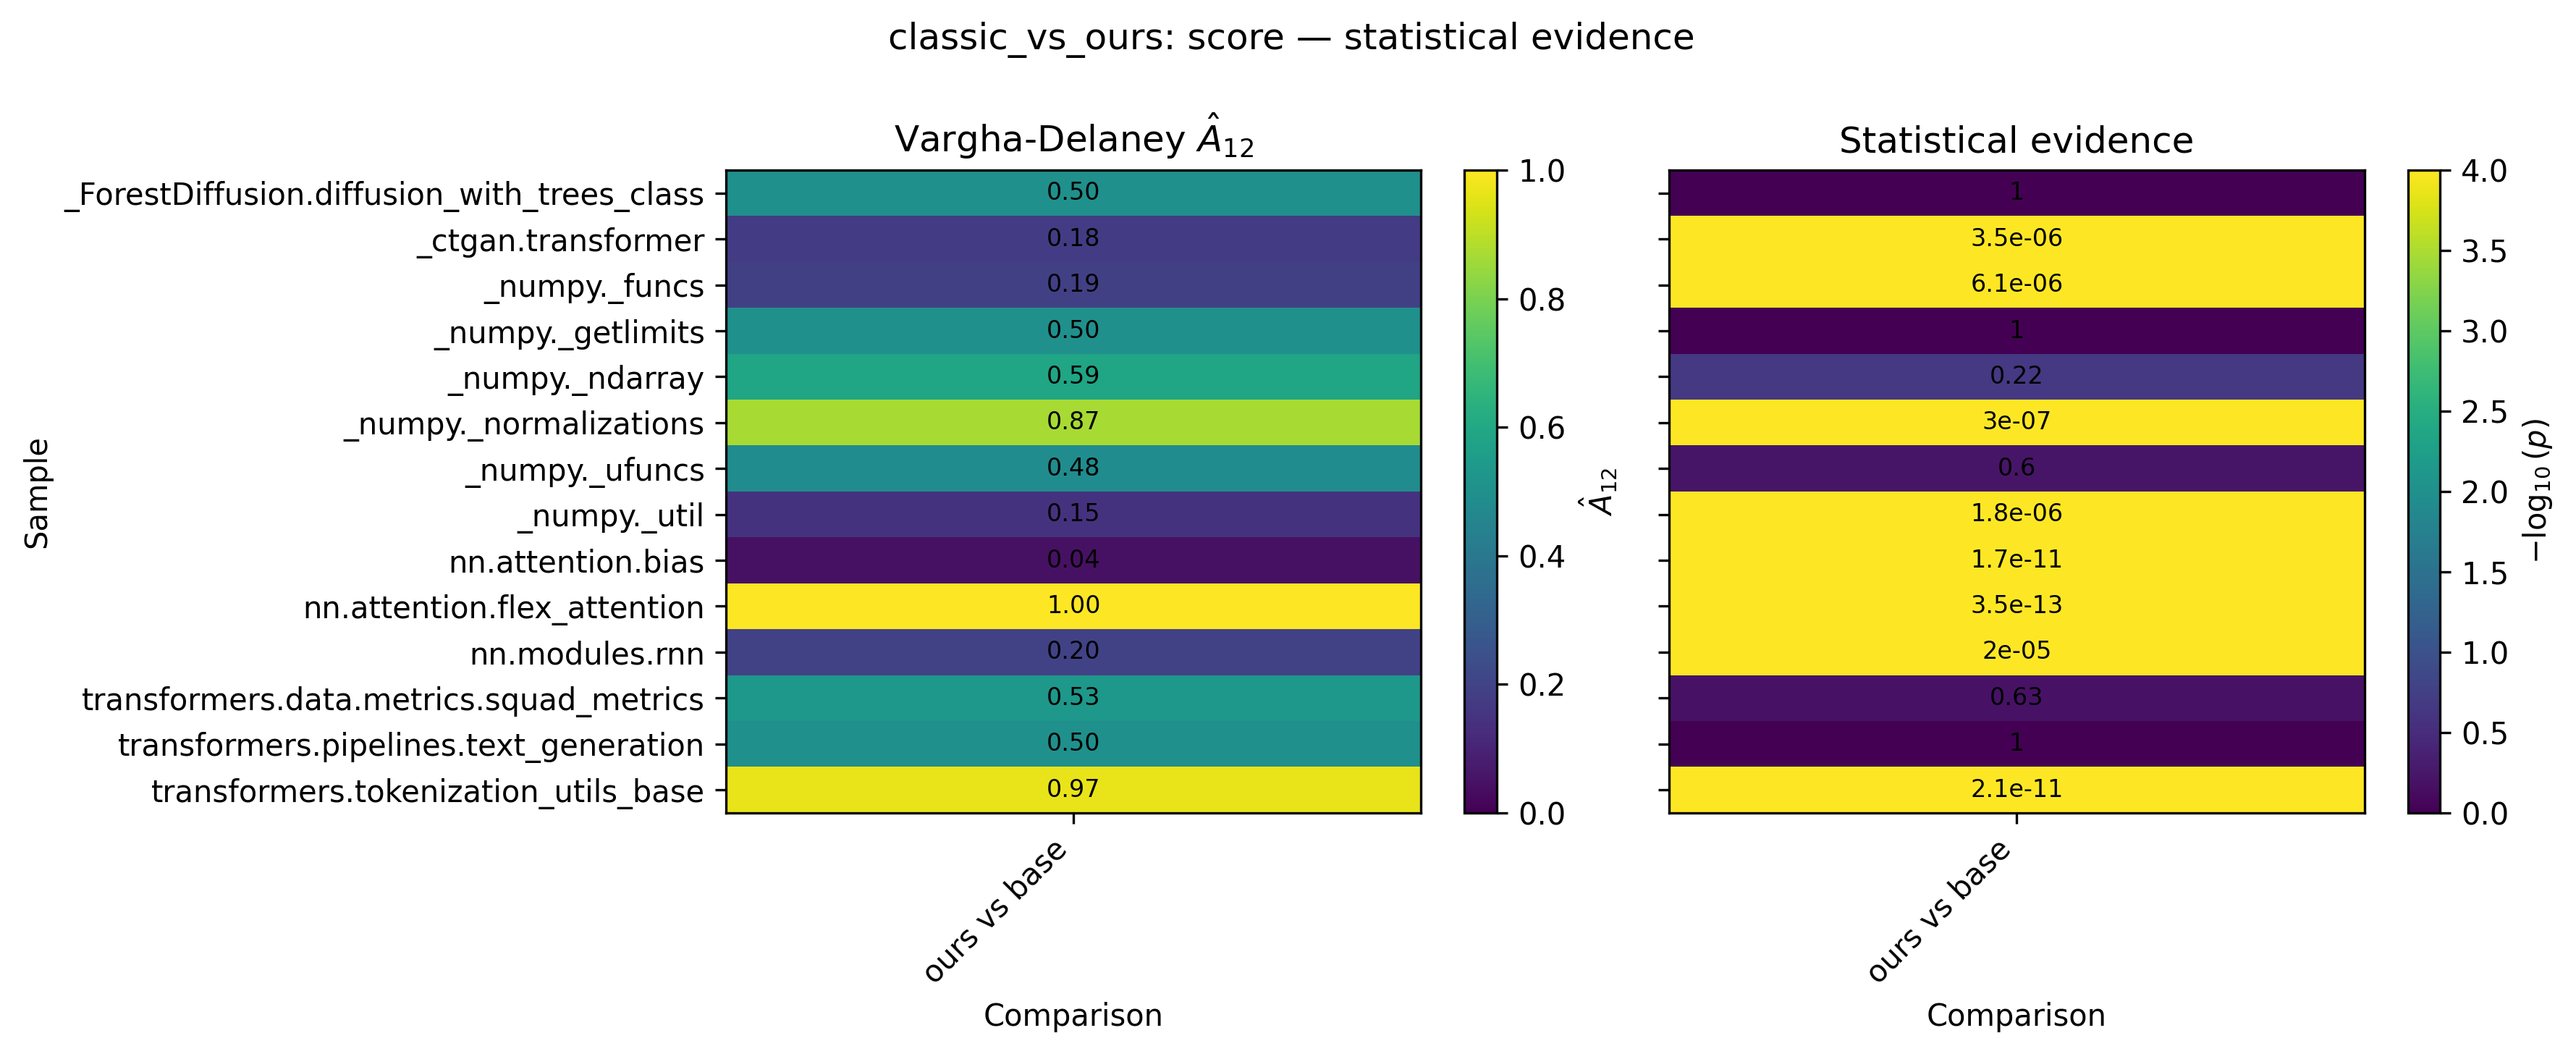
\includegraphics[width=\linewidth]{assets/classic_vs_ours_score_evidence.png}
    \caption{Distribution of coverage scores (classic baseline vs. new deserializer)}\label{fig:classic_vs_ours_dist}
\end{figure}

The results reveal a more nuanced picture than initially expected. On coverage scores, the baseline approach performs better on 6 out of 15 modules, while our new deserializer performs better on 5 modules, with 3 modules showing no significant difference. Of the 8 modules with statistically significant differences ($p < 0.05$), the baseline is superior on 5. Notably, our approach achieves large improvements on \texttt{nn.attention.flex\_attention} ($\hat{A}_{12} = 1.000$, large effect) and \texttt{transformers.tokenization\_utils\_base} ($\hat{A}_{12} = 0.967$, large effect). However, the baseline performs substantially better on modules such as \texttt{nn.attention.bias} ($\hat{A}_{12} = 0.045$, $p < 0.001$, large effect) and \texttt{numpy.\_util} ($\hat{A}_{12} = 0.146$, $p < 0.001$, large effect).

\begin{figure}[H]
    \centering
    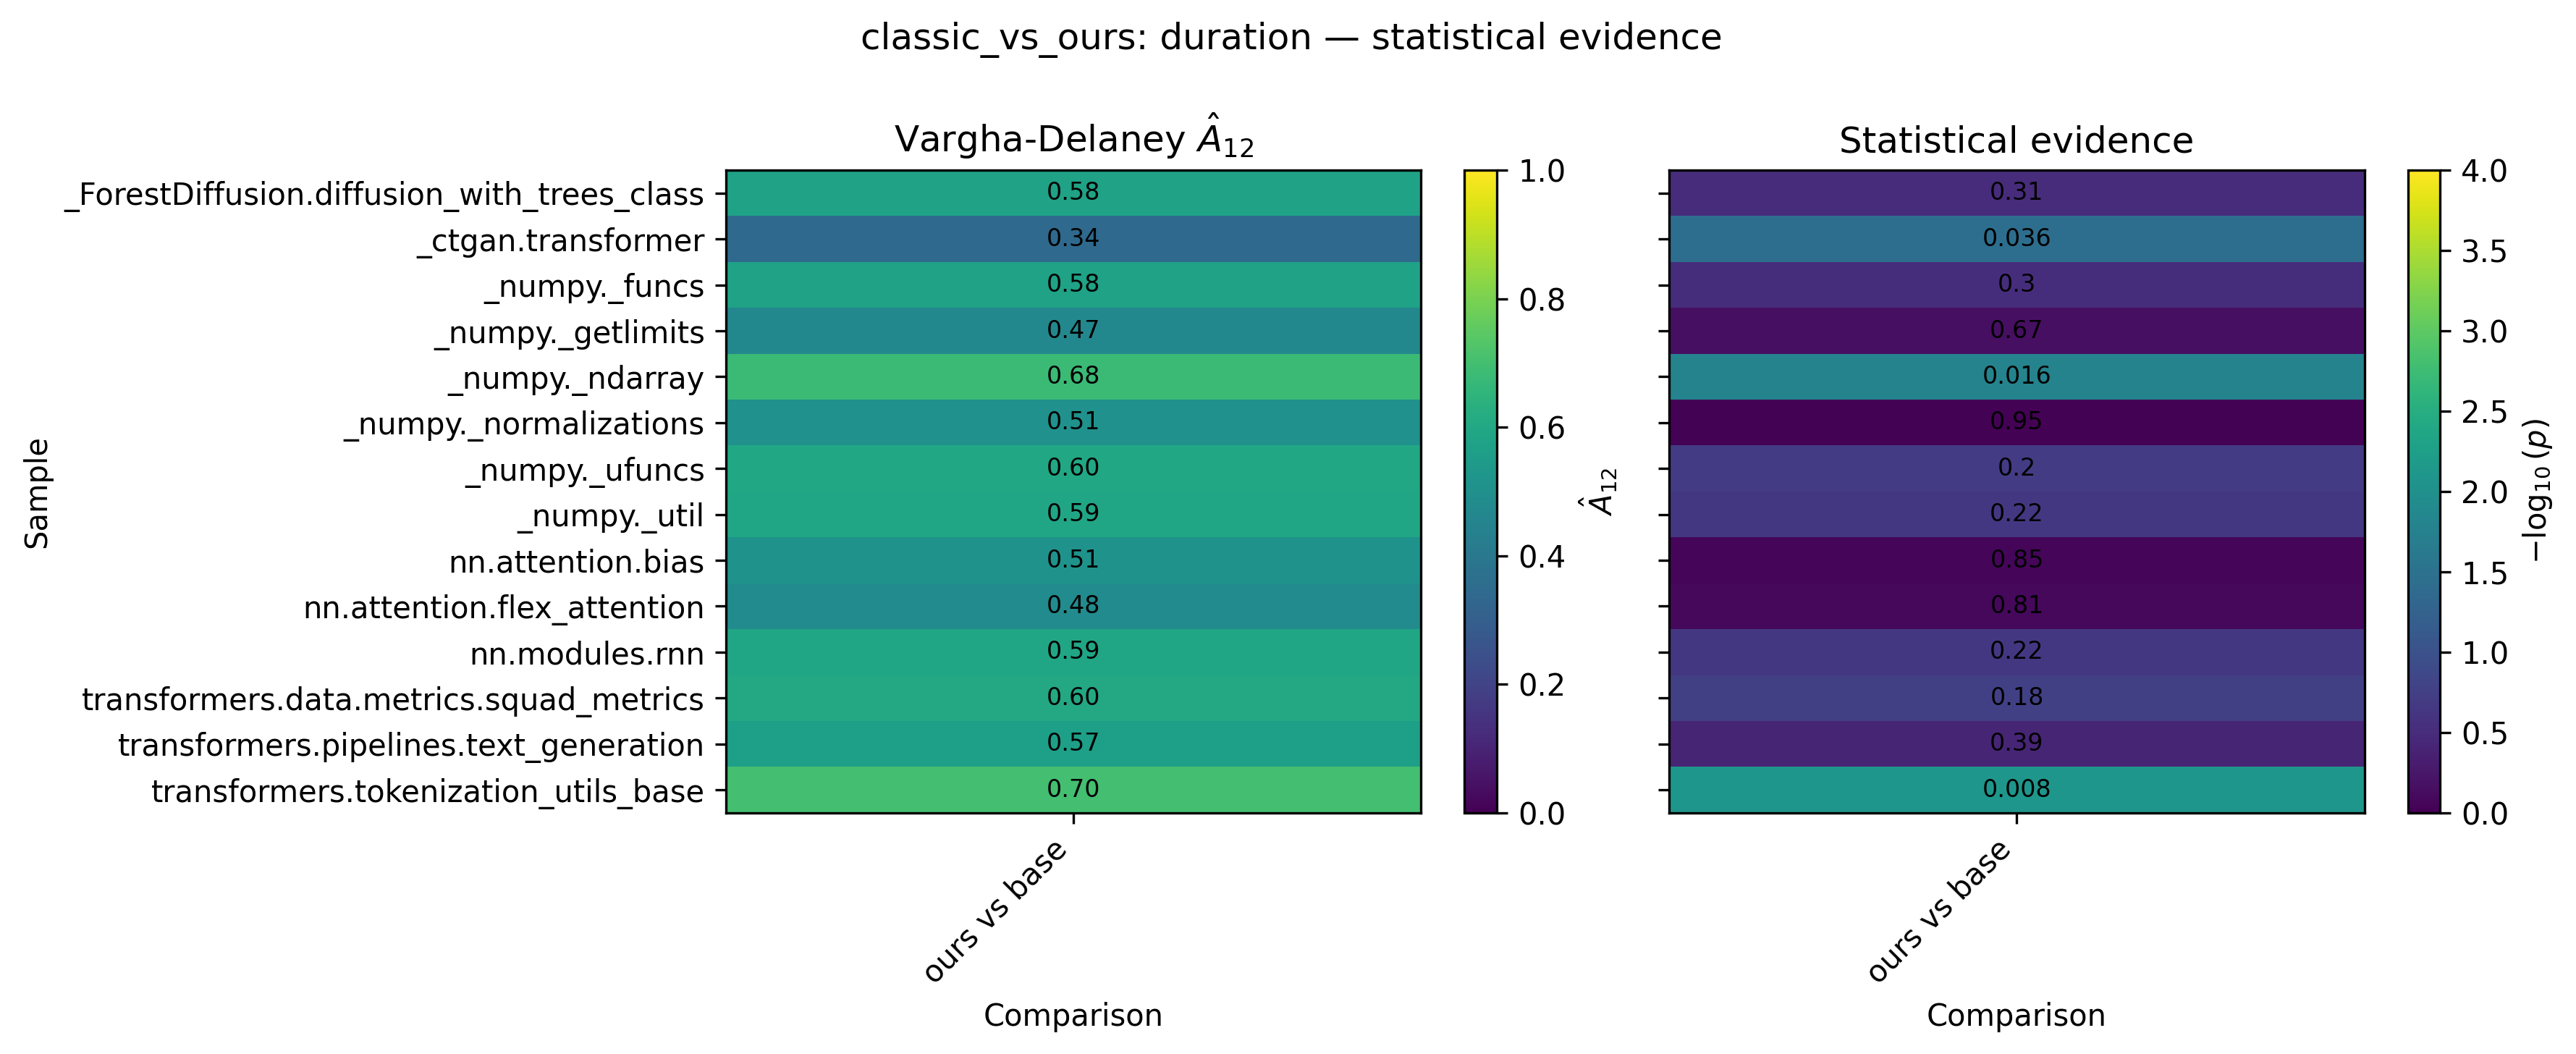
\includegraphics[width=\linewidth]{assets/classic_vs_ours_duration_evidence.png}
    \caption{Statistical evidence for deserializer comparison (duration)}\label{fig:classic_vs_ours_evidence}
\end{figure}

Results for execution time tend to favor our new deserializer, with 12 out of 15 modules showing faster execution times. However, the statistical significance of these differences is limited.

These mixed results suggest that while our improvements are beneficial for some modules (particularly those requiring complex test case construction), they do not uniformly outperform the baseline across all tested libraries. The improvements show their greatest benefit on modules with significant parsing demands, while the baseline approach remains more effective on others. This indicates that the effectiveness of deserialization improvements is heavily context-dependent and may require further investigation into which specific code patterns benefit most from our enhancements.

\subsubsection{Prompt engineering and context compression}

The new prompt (``UncoveredTargetsPrompt'') includes detailed instructions and context compression. We compare it both with the default prompt (``DefaultPrompt'') and with the same instructions without compression (``NoCompressionPrompt''), to measure their relative performance. Figure~\ref{fig:prompt_dist} shows the distribution of coverage scores for all three prompt strategies across the tested modules.

\begin{figure}[H]
    \centering
    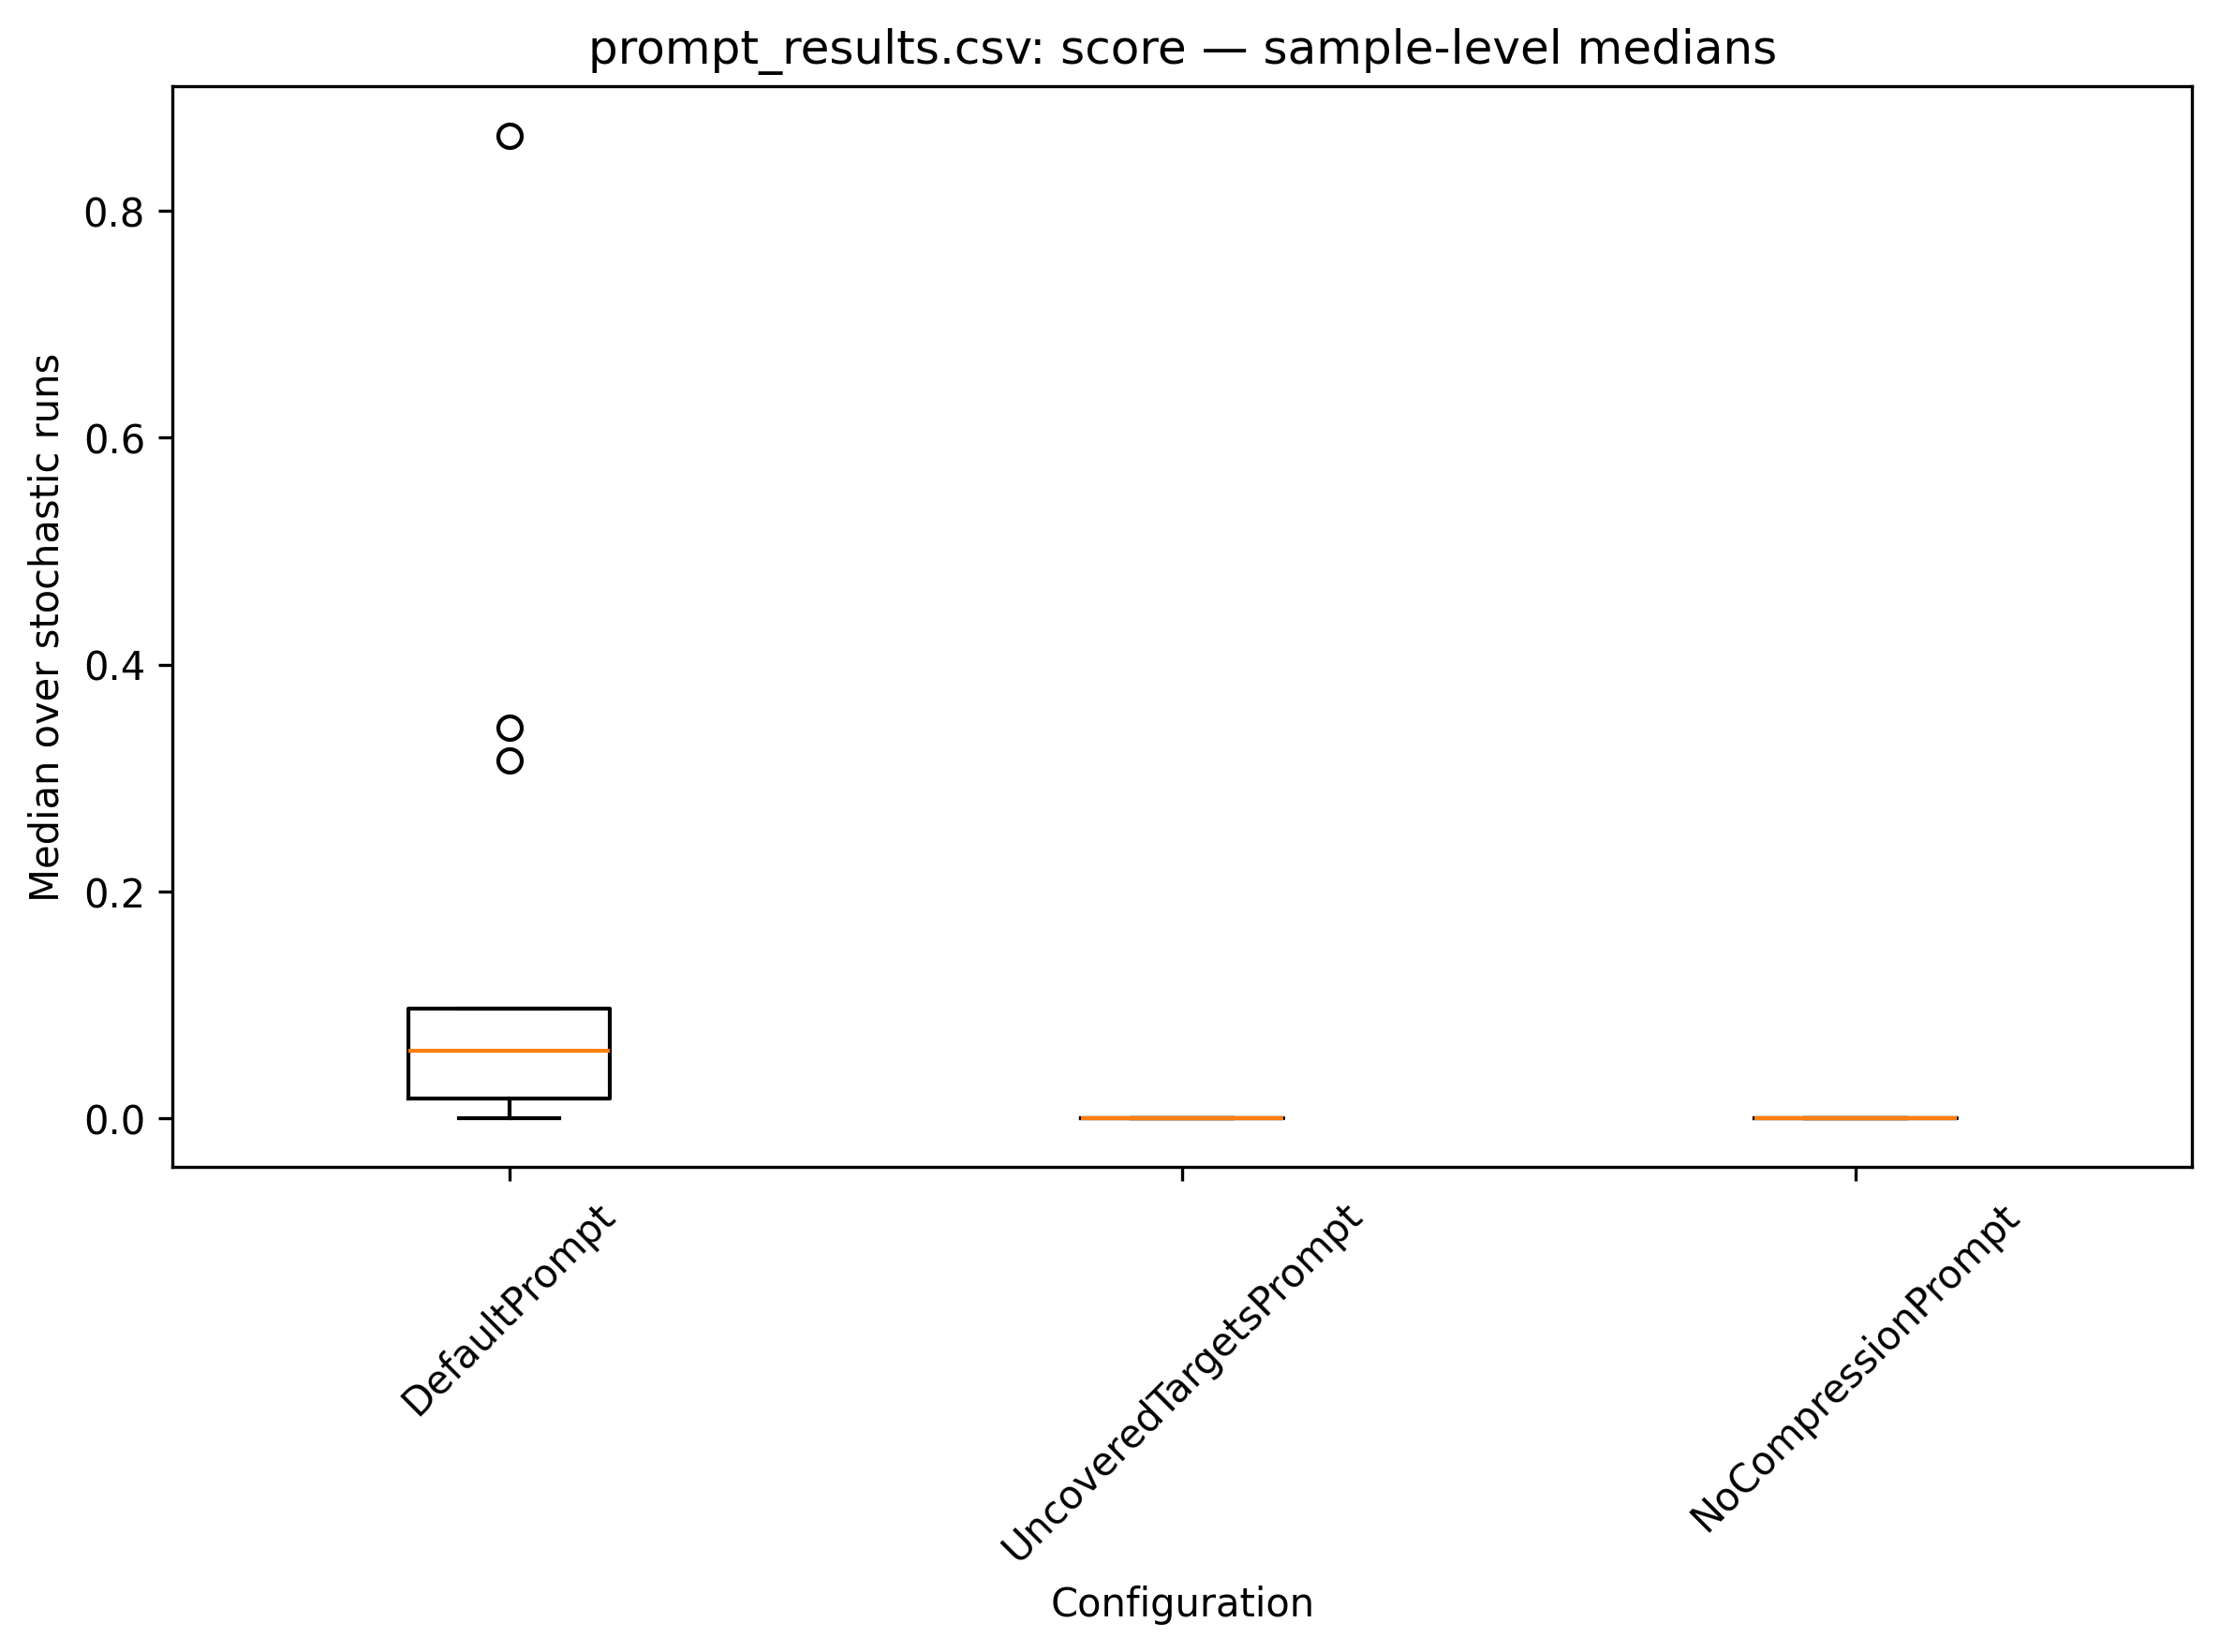
\includegraphics[width=0.75\linewidth]{assets/prompts_score_distribution.png}
    \caption{Distribution of coverage scores across different prompt strategies}\label{fig:prompt_dist}
\end{figure}

Contrary to expectations, the results demonstrate that the default prompt (``DefaultPrompt'') substantially outperforms the detailed prompt (``UncoveredTargetsPrompt'' and ``NoCompressionPrompt'') on most tested modules.

\begin{figure}[H]
    \centering
    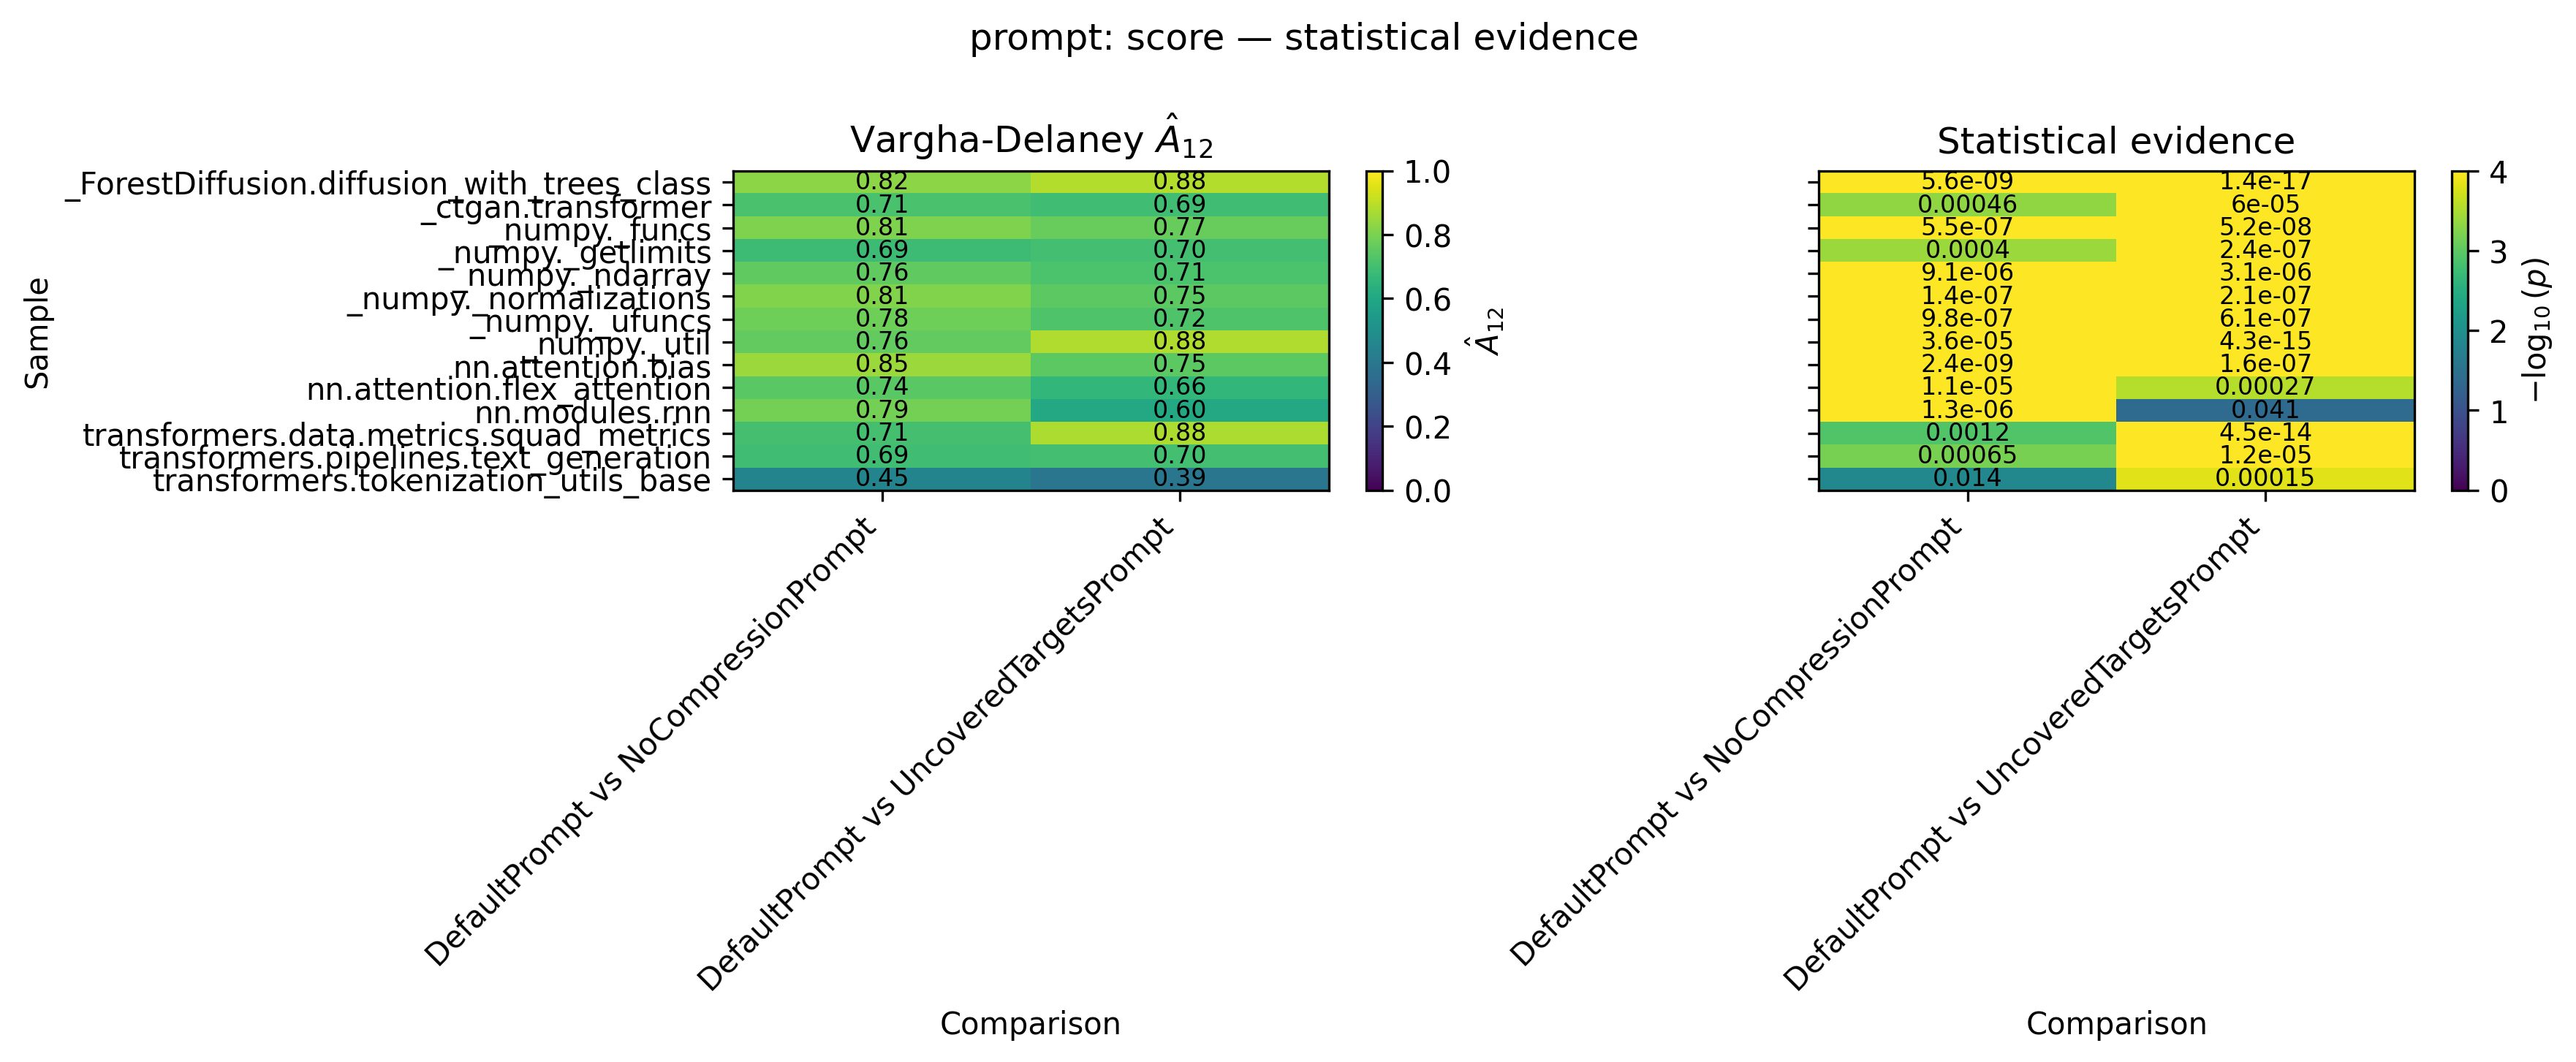
\includegraphics[width=\linewidth]{assets/prompt_score_evidence.png}
    \caption{Statistical evidence for prompt comparison (score coverage)}\label{fig:prompt_evidence}
\end{figure}

Regarding execution time, the compressed prompt can be compared directly with NoCompressionPrompt to isolate the cost of context compression, while the DefaultPrompt comparison captures the combined effect of changing the instructions and context. With NoCompressionPrompt as the left-hand configuration, the direct comparison gives a score $\hat A_{12}$ of 0.475 on average (median 0.451) across the 14 modules. The compressed prompt has the higher score in 9 modules, but only 3 of the 5 statistically significant comparisons favor compression; the other 2 favor no compression. Thus, compression alone does not produce a consistent coverage advantage. It does, however, substantially reduce execution time: compression is faster in 13 of 14 modules according to the A12 direction, with 7 statistically significant differences. The complete statistical output (Table~\ref{tab:prompt}) reports both metrics for every sample.

These results do not support the hypothesis posed in \ref{rq:prompt}. The default prompt remains substantially better for coverage than both alternatives, while compression mainly provides a runtime benefit. Comparing NoCompressionPrompt with UncoveredTargetsPrompt also shows that the loss in coverage cannot be attributed to context compression alone; and the detailed prompt reduces coverage on this benchmark.

\subsubsection{Model comparison}

To understand the effect of different language models on test generation performance, we compared multiple model variants across different model families and sizes. Figure~\ref{fig:models_dist} shows the distribution of coverage scores for different models.

The complete statistical output (Table~\ref{tab:coder_vs_non_coder} and Table~\ref{tab:model_weight}) provides a detailed view of the performance differences between the various model variants.

Model selection shows mixed effects on coverage performance. The 260 weight comparisons consist of 130 duration and 130 score comparisons. For coverage, only 8 comparisons have a large effect, and the median $\hat{A}_{12}$ is 0.500, indicating no general advantage for smaller or larger weights. In contrast, duration has 44 large effects, with a median $\hat{A}_{12}$ of 0.642 because the smaller model is always the left-hand configuration. The strongest and most consistent duration differences favor the smaller model, including Gemma 4 0.5b versus 12b on \texttt{transformers\allowbreak .data\allowbreak .metrics\allowbreak .squad\_metrics} ($\hat{A}_{12}=0.968$, large effect), where the 0.5b model executes much faster.

We also separately compared coder and non-coder Qwen models at matched weights. Across 20 comparisons (10 per metric), coder models show essentially no advantage in duration (median $\hat{A}_{12}=0.526$) and no advantage in coverage (median $\hat{A}_{12}=0.489$). The direction is not stable across weights: the 1.5b coder model has higher coverage on 8 of 10 modules, whereas the 3b coder model has higher coverage on only 4. Only 2 duration and 5 score comparisons are statistically significant, and none has a large effect. These results provide no evidence that the coder variant consistently improves coverage, nor does it show a consistent disadvantage.

The results therefore reveal a more specific trade-off than a simple model-size effect. Weight seems to have has a relationship with duration, but little systematic relationship with coverage. Coder tuning has no consistent effect on either metric in this dataset. Smaller models may consequently be preferred for more effecient ressource usage (time, computational or financial).

\subsection{Findings}

Our experimental evaluation reveals unexpected results that contradict our initial hypotheses:

\subsubsection*{Regarding \ref{rq:approach} (Deserializer improvements)}
The improvements to the LLM-to-test-case pipeline show mixed effectiveness. While our modifications enable the deserializer to handle additional Python constructs and improve robustness for certain edge cases (particularly \texttt{nn.\allowbreak attention.\allowbreak flex\allowbreak \_attention} and \texttt{transformers.\allowbreak tokenization\allowbreak \_utils\allowbreak \_base}), the baseline approach actually performs better on 6 out of 15 modules. It seems that while the improvements are beneficial for some modules, they do not consistently outperform the baseline across all tested libraries. This suggests that the effectiveness of deserialization improvements is context-dependent and may require further investigation into which specific code patterns benefit most from our enhancements.

Overall, in this dataset, we cannot conclude that our improvements to the deserializer consistently improve coverage. This indicates that while our enhancements are valuable for certain scenarios, they do not universally enhance test generation performance.

\subsubsection*{Regarding \ref{rq:prompt} (Prompt engineering and context compression)}
Contrary to expectations, the default prompt substantially outperforms the more detailed on most metric-sample comparisons. The additional ``UncoveredTargetsPrompt'' versus ``NoCompressionPrompt'' comparison allows the effects of context compression to be assessed separately from the effects of the revised instructions. Taken together, the results indicate that, in our specific case, giving more detail and guidance to the LLM actually \emph{reduces} coverage performance. The default prompt is simpler and more effective, while context compression mainly provides a runtime benefit without improving coverage. This experiment, however, was run only with the qwen2.5-coder:0.5b model (one of the lightest), and it is possible that other models may respond differently to the prompt changes. Further evaluation with different models would be needed to confirm the generality of this finding. We can conclude, however, that giving more detailed instructions to the LLM does not guarantee better performance, and that prompt design is a complex task that requires careful empirical evaluation.

\subsubsection*{Regarding \ref{rq:model} (Model selection)}
Model choice has limited systematic impact on coverage quality across our benchmark. Among the 260 weight comparisons, only 8 show large coverage effects and the median coverage $\hat{A}_{12}$ is 0.500. Weight does affect duration: 44 comparisons have large duration effects and the median duration $\hat{A}_{12}$ is 0.642 in favor of the smaller, left-hand model, although the 12b--26b Gemma comparison shows that this relationship is not strictly monotonic. Coder versus non-coder comparisons are similarly inconclusive: coder models have no large effects and show medians of 0.526 for duration and 0.489 for coverage. Smaller models can therefore be useful for reducing inference time, but neither size nor coder tuning consistently improves coverage.

\subsubsection*{Implications}
These results highlight the importance of empirical evaluation in LLM-assisted test generation research. Our intuitions about what would improve coverage—more detailed prompts, extended deserializer support, larger models—were not consistently validated. This suggests that LLM-assisted SBST is more complex than initially understood, with non-obvious interactions between components. The baseline approach, despite being simpler, proves to be more robust across diverse code characteristics. Future work should focus on understanding why the baseline approach is effective and identifying which specific code patterns would benefit from our enhancements, rather than assuming that more sophisticated approaches are universally better.


\subsection{Threats to validity}

Several limitations of this study should be noted:
\subsubsection{Internal validity}
The experimental setup uses 30 independent runs per configuration to account for the randomness inherent in both LLMOSA and the local LLM inference. However, the computational costs may introduce variability across different environments. The experiments were conducted on a compute cluster using Kubernetes, which provides isolation but does not completely eliminate environmental variations, such as hardware differences. Additionally, the choice of statistical test (Mann-Whitney U) assumes independence of observations.

\subsubsection{External validity}
Our evaluation focuses on 15 modules from three machine learning libraries (PyTorch, transformers, and TabGAN). While these represent popular and diverse libraries, the generalizability to other Python projects, particularly non-machine-learning codebases, remains uncertain. The modules were selected randomly to avoid bias, but the subset may not be fully representative of the broader ecosystem. Furthermore, the improvements to import resolution and deserializer robustness are tailored to handle specific patterns observed in machine learning libraries, and their effectiveness on other types of Python code is unknown.

\subsubsection{Construct validity}
We measure test generation effectiveness through two metrics: code coverage (measured as a score) and execution time. While these are standard metrics in the SBST literature and align with our research objectives, they do not fully capture test quality. Metrics such as fault detection ability or test maintainability are not evaluated. The coverage metric is provided by Pynguin's internal implementation and may be influenced by the specific instrumentation and branch coverage definitions used.

\subsubsection{Conclusion validity}
Statistical significance was determined using a the Mann-Whitney U test without correction for multiple comparisons. While this follows the recommendations of Arcuri and Briand~\cite{10.1145/1985793.1985795} for per-sample comparisons, the lack of multiple comparison correction increases the error rate across all comparisons.


\section{Conclusions}\label{sec:conclusion}
\subsection{Summary}

This paper investigates practical improvements to LLM-assisted test generation for machine learning libraries in Python, focusing on the interface between Large Language Models and the SBST algorithm LLMOSA in Pynguin. We implemented three key modifications: (1) an extensible LLM provider system enabling local, open-weight models through Ollama; (2) enhancements to the rewriter and deserializer, including improved import resolution and support for additional Python constructs; and (3) a more detailed prompt with context compression designed to guide LLM test generation.

Experimental evaluation on 15 modules from popular machine learning libraries reveals surprising findings that challenge common assumptions about LLM-assisted test generation. Contrary to expectations, the simpler default prompt substantially outperforms the enhanced prompt with detailed guidance (93\% of comparisons favor the default prompt), and our deserializer shows mixed results, showing no significant difference in most cases. Model selection has minimal impact on coverage, with larger models offering no significant advantage over smaller models, only increased inference latency.

These results highlight the importance of empirical evaluation and suggest that LLM-assisted SBST is more nuanced than initially anticipated. Rather than confirming that more sophisticated approaches uniformly improve performance, our evaluation demonstrates that the baseline approach, despite being simpler, provides better robustness across diverse code characteristics.

Due to not having substantial drops in coverage, smaller models may be more practical for real-world applications, offering comparable coverage with significantly  lower computational or financial resource consumption.

The findings suggest that simpler approaches seem to integrate more effectively with the SBST algorithm, pointing toward the need for careful investigation into which specific project characteristics benefit from targeted improvements, rather than applying complex modifications broadly.

\subsection{Future work}

Several promising directions for future work emerge from this study:

\begin{enumerate}
    \item \textbf{Parameter generation}: The parameter generation system (described in section~\ref{sec:approach}) remains incomplete. Finishing development and evaluating this component could further improve LLMOSA's ability to construct complex inputs required by machine learning APIs.

    \item \textbf{More extensive evaluation}: Evaluating the approach on additional machine learning libraries and domains would strengthen our analysis and identify library-specific improvements. The current evaluation is limited to 15 modules from three libraries, and a broader dataset could reveal patterns not captured in this study.

    \item \textbf{Hybrid approaches}: Investigating deeper integration between LLM-generated tests and the search algorithm, such as using the LLM to dynamically adjust search parameters or guide mutation strategies, could further improve coverage.

    \item \textbf{Cost-benefit analysis}: A more detailed analysis of the trade-offs between model size, inference cost, and coverage improvement could help developers select appropriate models for their use cases.
\end{enumerate}


\ifdetails
\subsection{Lessons learned}
Throughout this project, I sharpened my Python skills, improved my knowledge of Docker, especially how to optimize Dockerfiles for improved build speed, and learned how to use Kubernetes to deploy and manage containers in a compute cluster.
I followed the riguor and methodology of scientific research, reviewing the state of the art, identifying a problem, proposing a solution, and evaluating it. I had to conduct experiments in a reproducible manner, with proper documentation, replication, and statistical analysis. I also learnt how to write a scientific paper, and how to present my work clearly and concisely.
I was also able to attend a few presentations and thesis defenses, which gave me a better understanding of the research process and the challenges faced by researchers.
Finally, I improved my time management, prioritization skills and autonomy, which is crucial in research.
These lessons will be useful for my future career, as they are applicable to any research or development project alike.
\fi

\phantomsection{}
\section*{Acknowledgments}\label{sec:ack}
\addcontentsline{toc}{section}{\nameref{sec:ack}}
I would like to thank Xavier \textsc{Devroey} (my tutor) and Lucas \textsc{Berg} for providing valuable guidance during my internship.

Thanks as well to Paul \textsc{Temple}, and the whole SNAIL team for their support and feedback during the development of this work.

\ifdetails
\section*{Keywords}\label{sec:keywords}
\addcontentsline{toc}{section}{\nameref{sec:keywords}}
\emph{Software Testing, Search-Based Software Testing (SBST), Large Language Models (LLMs), Python, Pynguin, Ollama}
\fi



\newpage
\phantomsection{}  % Ensures hyperref links correctly to the references page
\addcontentsline{toc}{section}{References}
\printbibliography{}

\clearpage
\begin{appendices}

\ifdetails
\section{RSE de l'organisation d'accueil}
\begin{figure}[H]
\centering
    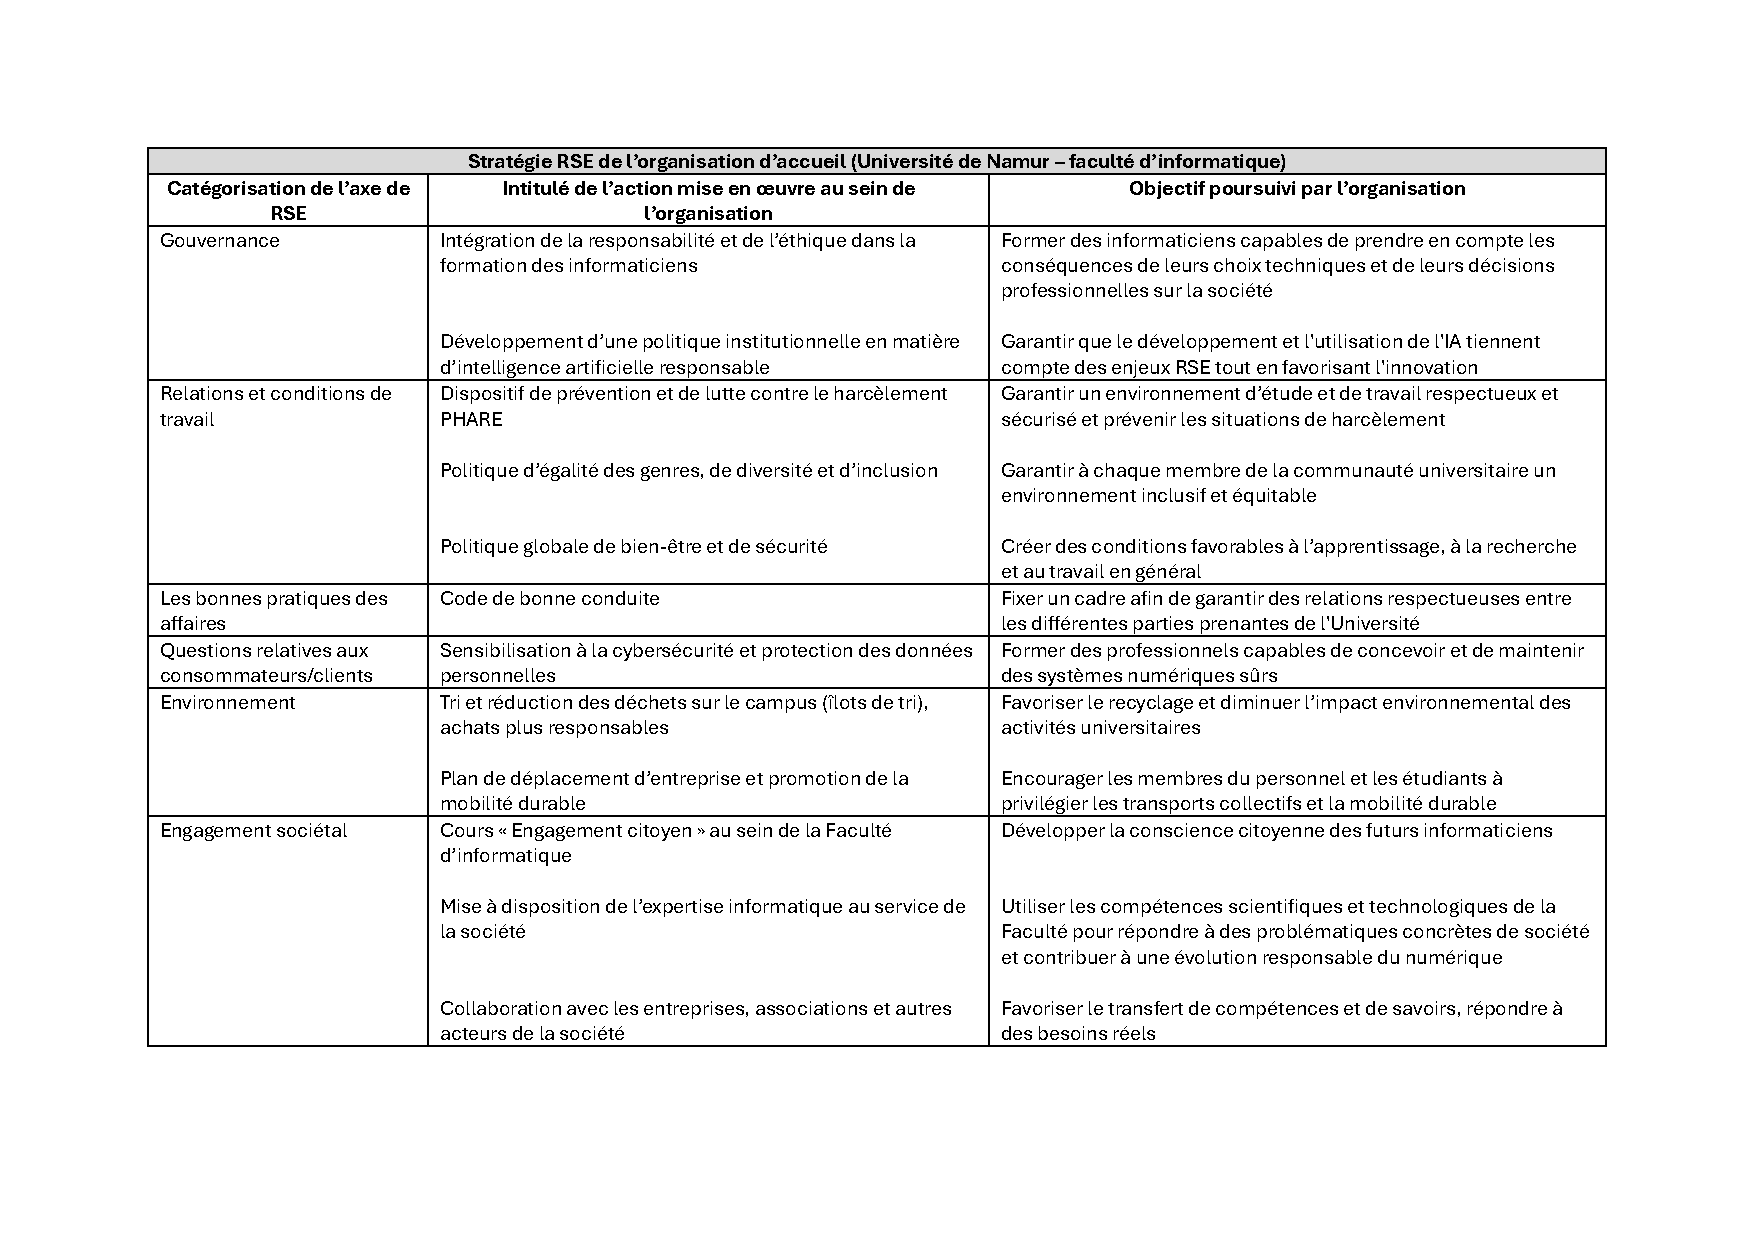
\includegraphics[width=\linewidth]{assets/Stratégie_RSE_UNAMUR.pdf}
    \caption{Stratégie RSE de l'université de Namur et de la faculté d'informatique}
\end{figure}
\fi
\section{Experiment results}

This appendix provides detailed results for all statistical comparisons conducted during the evaluation. The tables present comparisons using the Mann-Whitney U test's $p$-values with Vargha-Delaney $\hat{A}_{12}$ effect sizes.

\subsection{Deserializer}
\input{../analysis/out/classic_vs_ours.tex}

\subsection{Prompt comparisons}
\input{../analysis/out/prompt.tex}

\subsection{Model comparisons}
\input{../analysis/out/coder_vs_non_coder.tex}
\input{../analysis/out/model_weight.tex}
\begin{figure}[hbt]
\centering
    
\includegraphics[width=0.55\linewidth]{assets/model_score_value_distribution.png}
    \caption{Distribution of coverage scores across different LLM models \emph{(log scale)}}\label{fig:models_dist}
\end{figure}

\end{appendices}
\end{document}
